
\section{Apprentissage non paramétrique et analyses comparatives\label{sec:odometry_lwpr}}

Cette section présente nos premières expérimentions menées
sur la correction et l'apprentissage de l'odométrie ainsi que 
du modèle de déplacement sur nos petits robots humanoïdes.
Cette étude a donné lieu à la publication de l'article 
\cite{OdometryICRA2016}.

\subsection{Caractéristiques majeures de la méthode}

Comme mentionné précédemment, le problème de l'estimation
de l'odométrie et de la prédiction du déplacement sont fortement liés.
Les mêmes données expérimentales permettent d'étudier les deux problèmes.
Cependant, ces deux sujets ne sont que rarement traités ensembles dans 
la littérature et encore moins comparés selon les mêmes conditions.

Chez les robots à roues, la simplicité du déplacement fait que le
même modèle de déplacement est utilisé dans les deux cas.
La calibration de l'odométrie revenant alors la plupart du temps 
à l'identification des paramètres du modèle de déplacement.

Pour les robots à pattes et humanoïdes, le système mécanique 
est sous actué relativement à son déplacement sur le sol et 
les deux problèmes sont séparés.
Chez l'humanoïde l'odométrie est estimée soit directement à partir des informations
proprioceptives et du modèle géométrique sans calibration, soit à l'aide 
de techniques d'analyse visuelle.

Ici, l'estimation de l'odométrie et la prédiction du déplacement sont
à la fois étudiées et comparées.

\begin{itemize}
    \item La précision de l'odométrie proprioceptive et la prédiction du 
        déplacement du robot sont toutes les deux étudiées et comparées.
        Cette comparaison des deux problèmes \textit{dans les mêmes conditions} 
        est très rarement présentée dans la littérature.
    \item L'odométrie des robots humanoïdes tend de plus en plus à être estimée 
        par des techniques visuelles. 
        Néanmoins, les travaux présentés ici prennent le parti de ne pas s'appuyer sur 
        le traitement d'image. 
        Les méthodes de correction et de calibration de l'odométrie
        mises aux points sur les robots à roues sont ici appliquées 
        aux robots humanoïdes.
    \item L'odométrie proprioceptive reste à la base de nombreux autres
        procédés de localisation dont l'odométrie visuelle.
        Les travaux présentés ici sont destinés d'une part à améliorer la précision 
        des techniques de localisation et d'autre part à réduire l'effort d'asservissement 
        afin de suivre une trajectoire planifiée.
    \item Puisque n'utilisant pas d'analyse d'image, les temps de calculs de l'odométrie 
        après apprentissage sont faibles.
        Même sur l'ordinateur embarqué du robot, la correction peut se faire 
        à la fréquence de la boucle de mise à jour bas niveau.
    \item Notre méthode propose la construction d'une fonction de correction
        modélisant les différences entre les déplacements souhaités ou 
        les déplacements proprioceptifs mesurés et les déplacements réels du robot.
        Les modèles cinématiques utilisés sur robots à roues sont très majoritairement linéaires. 
        Ici, le choix à été fait de ne pas poser d'apriori sur la forme de la fonction de correction.
        Au lieu d'employer un modèle linéaire ou plus généralement un modèle paramétrique, 
        une technique d'apprentissage non linéaire et non paramétrique est testée.
    \item L'évolution des règles de la compétition RoboCup a introduit
        à partir de 2015 une nouvelle surface de jeu dans la ligue humanoïde.
        La moquette verte du terrain a été remplacée par de l'herbe artificielle. 
        Cette surface plus \textit{molle} affecte grandement la locomotion des robots. 
        Une comparaison de l'odométrie et de la prédiction du déplacement 
        est alors mené sur ces deux surfaces.
    \item Le générateur de marche utilisé au cours des expérimentations sur le robot
        Sigmaban est détaillé dans la section \ref{sec:walk}. 
        L'effet sur la locomotion du processus de stabilisation 
        utilisant les capteurs de pression est également analysé
        au travers de son influence sur l'odométrie.
    \item La méthode proposée repose en grande partie sur l'emploi d'un
        système de capture de mouvement externe capable de mesurer avec
        une grande précision la pose du robot tout au long de son déplacement.
\end{itemize}

\subsection{Méthodes de régression non paramétriques\label{sec:odometry_non_parametric}}

Il n'y a pas de définition universellement reconnue permettant une distinction 
précise entre les méthodes paramétriques et non paramétriques.
Cette catégorisation est ambigüe et est pour beaucoup une 
question de point de vue relatif à l'application des différentes méthodes.
Nous adoptons néanmoins ici la séparation suivante.

Les méthodes de régressions paramétriques imposent la forme du modèle recherché.
L'intérêt de ces modèles est de permettre au concepteur d'injecter
dans la modélisation la connaissance experte du problème considéré.
Chaque élément de l'ensemble des paramètres du modèle peut
alors être interprété et fournit un renseignement 
sur les propriétés du système.
Le modèle de la régression linéaire et le modèle géométrique direct
des robots sont tous deux des modèles paramétriques.

A l'inverse, les modèles non paramétriques n'imposent pas de forme a priori.
La grande majorité de ces méthodes supposent néanmoins que la fonction
recherchée sous-jacente possède une certaine régularité (\textit{smoothness}).
Ces régressions sont ainsi plus flexibles et ne requièrent que peu de 
présupposés sur le problème.
Mais en contre partie, comme la forme de la solution est directement extraite
des données, elles en nécessitent une bien plus grande quantité.
De plus, les données expérimentales ne sont jamais exemptes de bruit et
la gestion du compromis biais variance revêt une importance particulière.
Souvent, les méthodes non paramétriques laissent la possibilité au concepteur 
d'ajuster la complexité du modèle construit.
Il est ainsi essentiel d'avoir un a priori sur le caractère lisse 
de la fonction recherchée. 
Le principal risque étant le surapprentissage (\textit{overfitting}).\\

Les techniques de régressions non paramétriques ont une longue histoire 
(\cite{hardle_applied_1990}, \cite{yatchew_nonparametric_1998}).
Elles sont utilisées dans de nombreux domaines et de multiples 
approches ont été développées\footnote{Cette liste illustre la diversité des méthodes 
de régressions non paramétrique. Elle ne saurait être exhaustive.}, 
dont beaucoup partageant des idées proches :
\begin{itemize}
    \item Un pan entier des modèles non paramétriques est représenté par 
        les approximateurs de fonctions.
        Par exemple, les réseaux de neurones (\textit{Neural Network}) (\cite{rojas_neural_2013}), 
        les splines polynomiales (\cite{durrleman_flexible_1989}, \cite{eubank_nonparametric_1999})
        ou encore les réseaux à fonctions de base radiale 
        (\textit{Radial Basis Function Network}) (\cite{park_universal_1991}).
        Le point commun de ces différentes méthodes est qu'elles possèdent toutes un ensemble 
        de méta paramètres contrôlant la complexité du modèle construit.
        Par exemple respectivement le nombre de couches et le nombre de neurones de chaque couche d'un perceptron, 
        le nombre de polynômes utilisés, leur degré et la position des recollements ou encore le nombre 
        et la position des fonctions de base radiale.
        Le choix de ses méta paramètres doit être fait de manière experte par le concepteur et
        dépend fortement du problème considéré.
    \item Les méthodes d'estimation par noyaux (\textit{kernel}) et des $k$ plus 
        proches voisins (\cite{ltman_introduction_1992}) sont typiquement représentatives
        de la régression non paramétrique. Dans ces méthodes, il n'y a pas d'étape d'apprentissage.
        L'évaluation en un point de la fonction construite se base directement sur les 
        données d'apprentissage.
        À chaque requête, les données d'entrées sont pondérées et moyennées selon leur distance 
        au point évalué.
        Le nombre $k$ ou la largeur du noyau contrôle le lissage de la fonction recherchée.
    \item Les processus gaussiens (\textit{gaussian process}, GP) popularisés dans le domaine 
        de l'apprentissage automatique par \cite{rasmussen_gaussian_2006} représentent un champ 
        de recherche très actif. Ils adoptent un formalisme bayésien et reposent sur
        une base statistique théorique fondée. 
        Ils ont ainsi pour avantage une modélisation complète de l'incertitude, 
        une très bonne vitesse de convergence (efficacité dans l'utilisation des données) 
        et leurs méta paramètres peuvent être automatiquement réglés.
        Malheureusement, les algorithmes d'apprentissage et d'évaluation sont respectivement cubique 
        et quadratique en la taille des données d'entrées.
        C'est l'amélioration de cette complexité qui motive ce domaine 
        de recherche (subdivision de l'espace, matrices creuses, ...).
        Sans cela, la malédiction de la dimension restreint leurs applications 
        à de faibles dimensions\footnote{Les processus gaussiens ont néanmoins 
        fait leurs preuves sur des problèmes \og simples \fg. L'exemple le plus connu, PILCO, 
        réalise l'apprentissage du modèle dynamique et le contrôle d'un pendule inversé physique
        (\cite{deisenroth_pilco:_2011}) en un très peu d'itérations.}.
    \item Une autre approche mélange les idées des méthodes à noyaux et des régressions 
        paramétriques classiques : les techniques de régressions pondérées locales 
        (\textit{locally weigthed regression} décrit par \cite{cleveland_locally_1988}
        et \cite{christopher_locally_1997}. 
        L'espace d'entrée est subdivisé en petites régions de la même manière que les noyaux. 
        Dans chacune de ces régions locales est ajusté un modèle paramétrique linéaire, 
        ne considérant que les points d'apprentissage contenus dans la région.
        Lors de l'évaluation d'un point, une pondération des différents modèles locaux est
        calculée selon la distance à leur zone locale (les régions locales peuvent s'intersecter).
        Ces méthodes permettent avec l'utilisation de modèles paramétriques d'améliorer l'extrapolation
        dans les zones où peu de données ont été récoltées. De plus, en ajoutant une phase d'apprentissage
        pour la construction des modèles locaux, l'évaluation d'un point n'est plus linéaire en la taille 
        des données d'entrée ; mais linéaire en le nombre de modèles locaux.
    \item Toujours avec l'idée de découper l'espace d'entrée, les arbres de décisions 
        ne subdivisent l'espace que selon des hyperplans alignés avec les axes de l'espace.
        De plus, les feuilles de ces arbres (représentant donc un hyperrectangle de l'espace) contiennent
        également un modèle de régression paramétrique. 
        Lors de l'évaluation, les arbres de décisions retournent la valeur calculée selon 
        le modèle de la feuille correspondant au point de l'espace recherché.
        Enfin, les arbres de décisions sont en réalité regroupés en forêt aléatoire (\textit{random forest}).
        Chaque arbre construit une subdivision de l'espace différente aléatoirement et les résultats 
        des multiples modèles (correspondant au même point de l'espace) 
        sont moyennés (\cite{liaw_classification_2002}).
    \item On peut également cité l'exemple de \cite{nguyen-tuong_model_2009} développant une méthode
        à mi chemin entre les processus gaussiens et la régression locale pondérée.
        Au lieu d'utiliser un simple modèle linéaire dans les régions locales, 
        des processus gaussiens sont employés.
        L'intérêt de ces travaux est de proposer une solution plus bien performante en terme de temps de calcul
        que les processus gaussiens (car le nombre de points d'apprentissage dans chaque région est faible) 
        mais dont la régression est néanmoins plus précise qu'en utilisant des
        modèles linéaires (mais aussi un peu plus lent).\\
\end{itemize}

Dans cette étude, le choix de la technique de régression non paramétrique 
c'est porté sur LWPR : \textit{Locally Weighted Projection Regression} ou 
régression par projection pondérée locale. Elle est présentée et détaillée 
par \cite{vijayakumar_incremental_2005}.
Comme sont nom l'indique, elle appartient à la famille des régressions pondérées locales
et est considérée comme la méthode état de l'art de ce domaine de recherche.
Son intérêt est d'être spécifiquement tournée vers la robotique et les applications
en temps réel. 
Les auteurs démontrent son efficacité en apprenant en temps réel et en ligne le
modèle dynamique inverse du bras d'un robot humanoïde à 30 degrés de liberté.
L'algorithme est exécuté sur le petit ordinateur embarqué du robot \textit{SARCOS}.
Ce modèle dynamique permet de contrôler en couple les moteurs du bras et donc d'améliorer 
la précision du suivi de trajectoire.

LWPR fonctionne en subdivisant l'espace d'entrée en régions locales appelées 
\textit{champs récepteurs} (\textit{receptive field}) au moyen de noyaux gaussiens. 
Chaque champ récepteur est alors défini par le vecteur de son centre dans l'espace 
d'entrée et sa matrice de covariance représentant sa taille selon les différentes dimensions.
Dans chacun de ces champs récepteurs, la régression aux moindres carrés partielle 
(\textit{Partial Least Square}, PLS) (\cite{wold_pls-regression:_2001}) est employée
à la place d'une régression linéaire classique.
Cette technique initialement développée dans le domaine de l'analyse de composés chimiques 
a pour particularité de calculer à la fois une régression linéaire et une 
réduction de dimension. 
Plus précisément, cet algorithme effectue de manière itérative une régression
linéaire simple et univariée en projetant les données d'apprentissage sur un axe 
particulier de l'espace d'entrée.
Cet axe est choisi afin de maximiser la covariance entre les données d'entrées 
projetées sur cet axe et la variable de sortie.
L'opération est alors répété sur les résidus de cette régression linéaire.

C'est grâce à cette réduction de dimension réalisée dans chacun des 
champs récepteurs que les auteurs parviennent à travailler sur des espaces 
de grande dimension.
Ils insistent sur le fait que dans la majorité des cas, le modèle dynamique des robots 
que l'on cherche à apprendre est en réalité un sous espace (\textit{manifold}) 
de dimension faible mais plongé dans un espace d'entrée 
de grande dimension (ici $30\times3=90$).

Un autre élément particulier de cette méthode LWPR est que l'apprentissage est incrémental.
Les points d'apprentissage sont fournis à l'algorithme un à un séparément ; 
permettant un apprentissage \og en ligne \fg pendant le fonctionnement du système
sans la nécessité de rassembler toutes les données en un seul paquet (\textit{batch}).
À chaque nouveau point d'apprentissage, l'algorithme met à jour 
la taille des champs récepteurs, ajoute si besoin de nouveaux champs 
et recalcule les régressions sans avoir besoin de stocker l'intégralité
des points déjà fournis.

Une des grandes raisons de la popularité de LWPR réside dans le fait que les auteurs ont 
mis à disposition une implémentation ouverte en C ainsi que des interfaces pour C++, MATLAB et Python. 
Cette implémentation est présenté dans l'article \cite{klanke_library_2008} et se retrouve
à l'adresse : \url{http://wcms.inf.ed.ac.uk/ipab/slmc/research/software-lwpr}

LWPR possède deux principales limites. 
Premièrement, bien que beaucoup plus rapide que les autres méthodes non paramétriques 
état de l'art comme le compare \cite{nguyen-tuong_model_2009},
ses performances d'ajustement (\textit{fitting}) sont également moindre.
De plus, la méthode requière de multiple méta paramètres dont certains très dépendants 
du problème d'apprentissage considéré et qui ne peuvent être réglés automatiquement.
Même si les auteurs fournissent une liste de conseils et d'étapes, une délicate 
phase manuelle d'essai-erreur est néanmoins nécessaire afin d'obtenir 
des résultats satisfaisant.\\

Pour résumé, l'utilisation d'un système de capture de mouvement nous permet
de nous reposer sur une méthode non paramétrique nécessitant une quantité de données
importante mais ne demandant que très peu d'a priori sur la fonction recherchée.
L'algorithme LWPR est choisi pour d'une part, son implémentation 
disponible mais surtout pour ses très faibles temps de calcul en comparaison 
de sa performance et des autres techniques disponibles.
Nos petits robots possèdent une puissance de calcul embarquée 
très limitée et la technique d'odométrie proposée est avant tout conçue 
pour servir de base à d'autres méthodes plus \og haut niveau \fg.
Le temps de calcul est ainsi pour nous primordial et LWPR est de loin 
l'algorithme le plus rapide en comparaison de ses performances.

\subsection{Système de capture de mouvement\label{sec:odometry_mocap}}

\begin{figure}[htbp]
    \begin{center}
        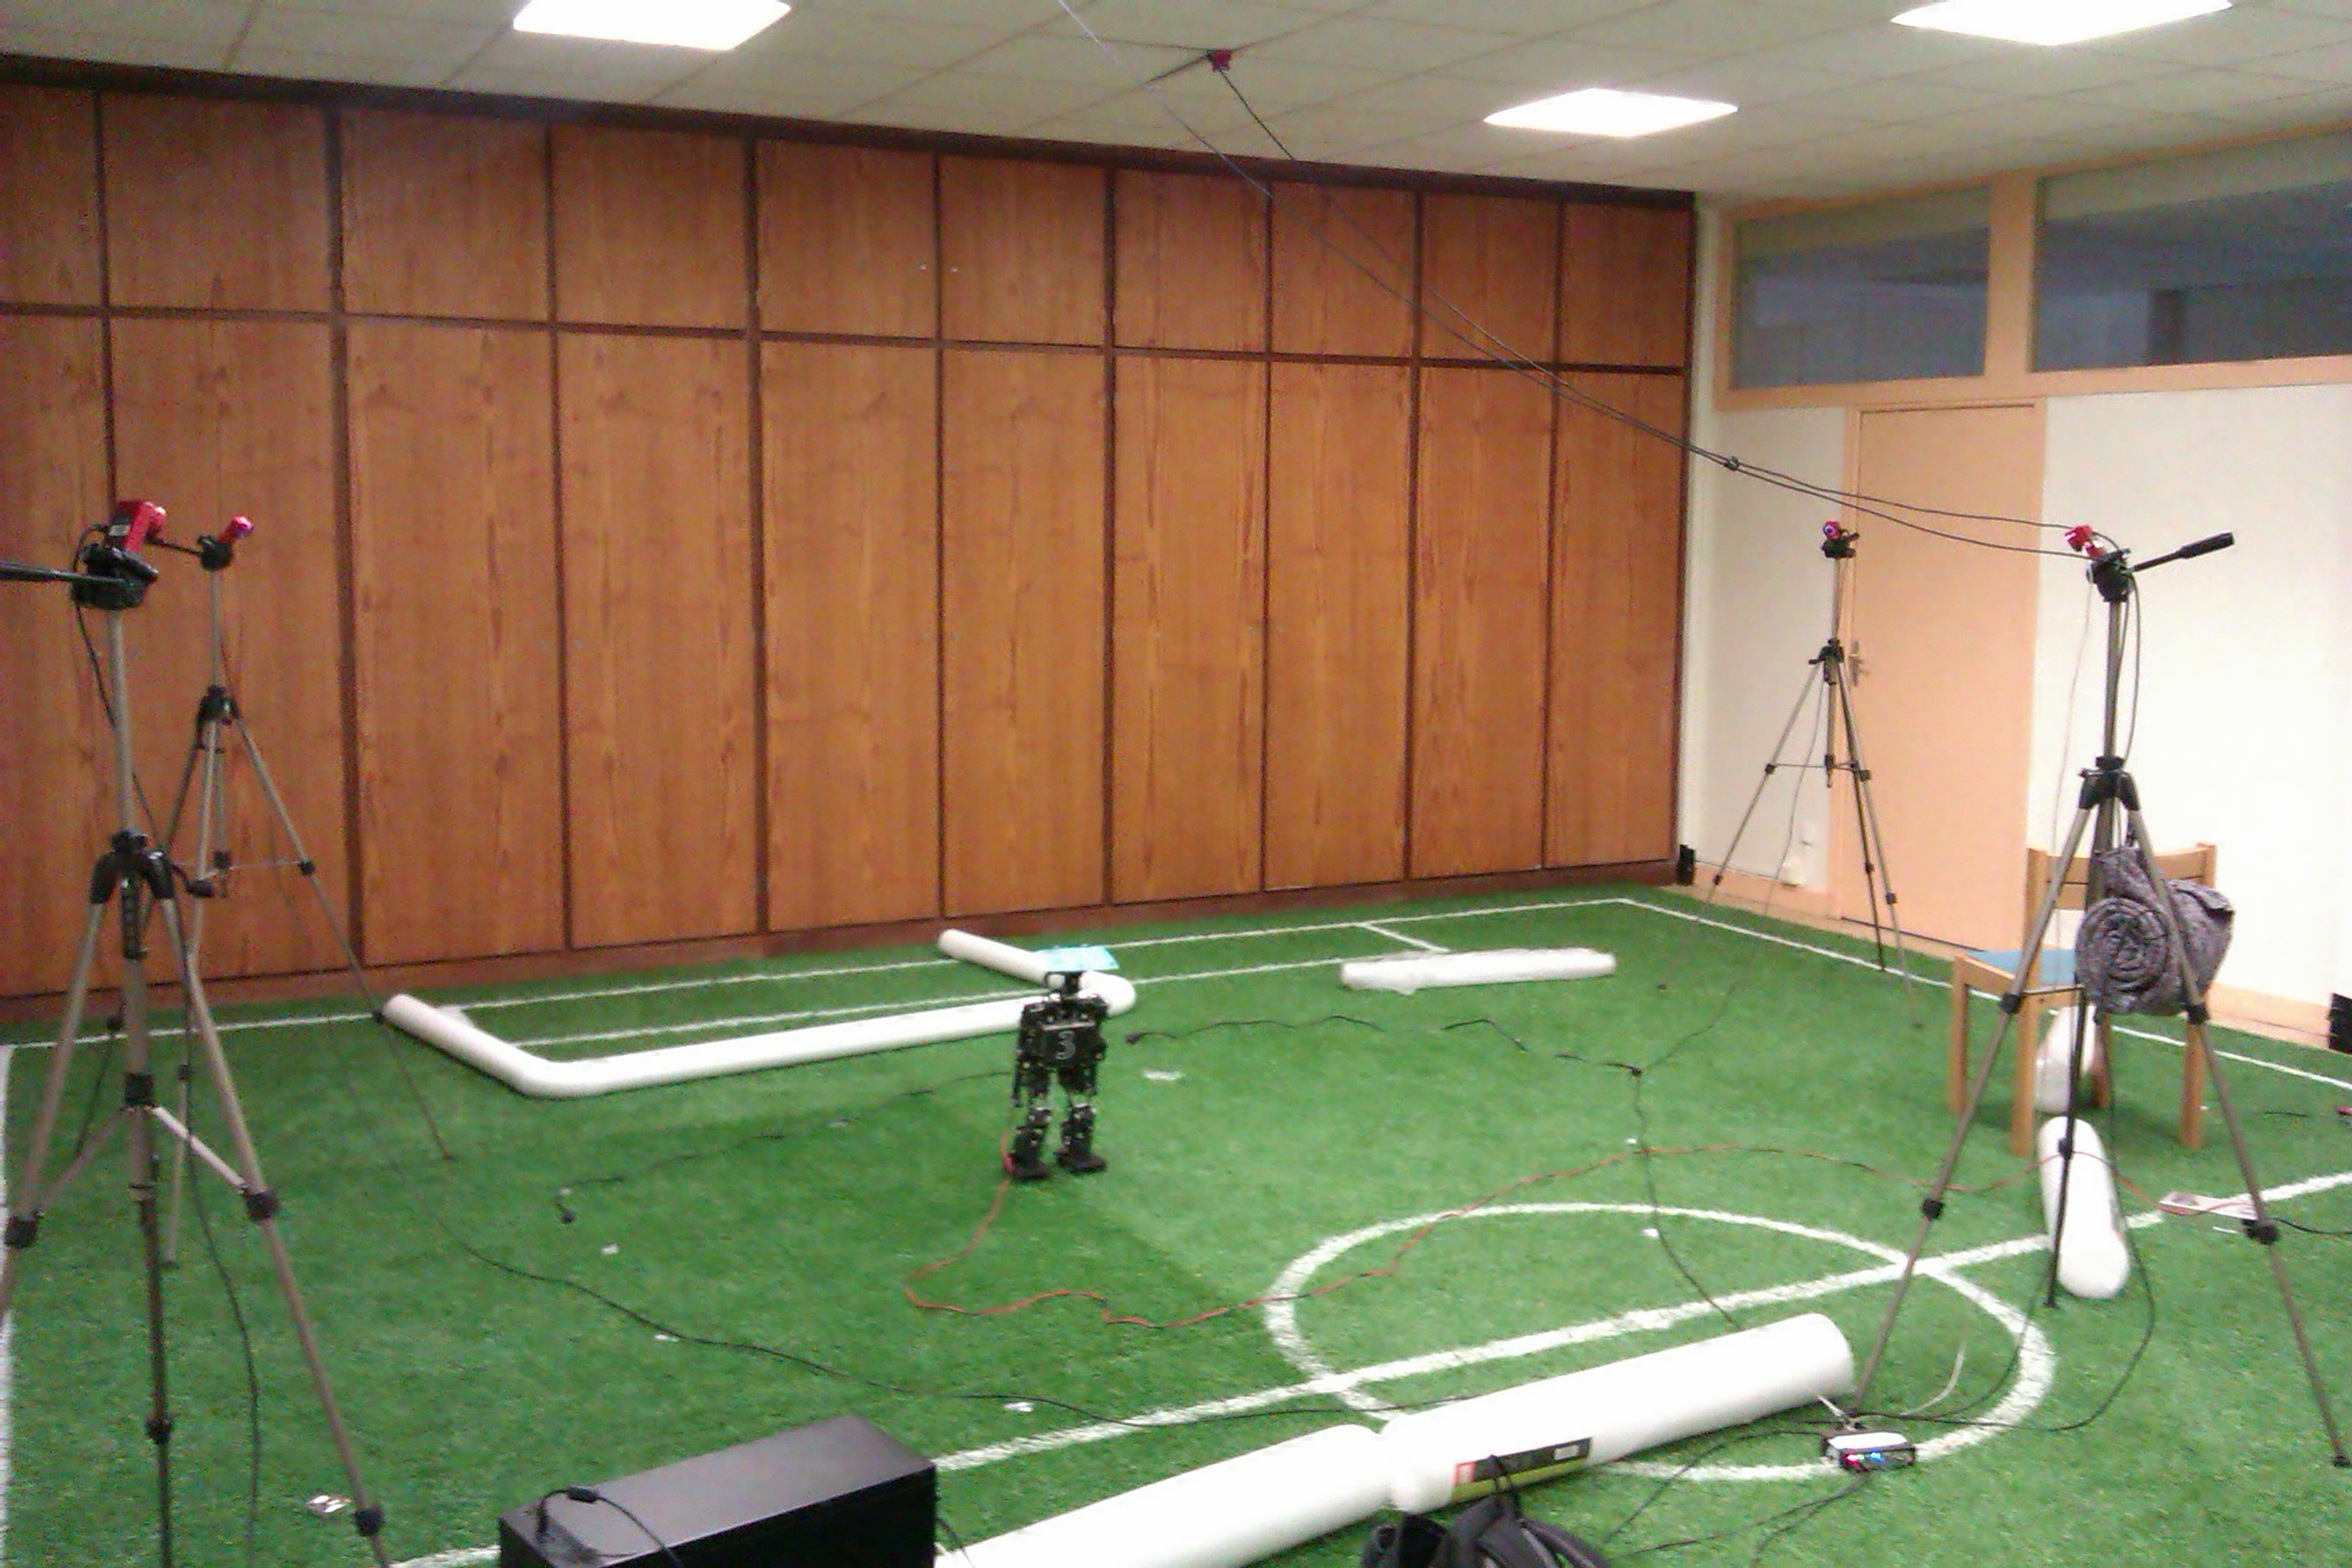
\includegraphics[width=0.8\linewidth]{../media/mocap_setup1.jpg}
        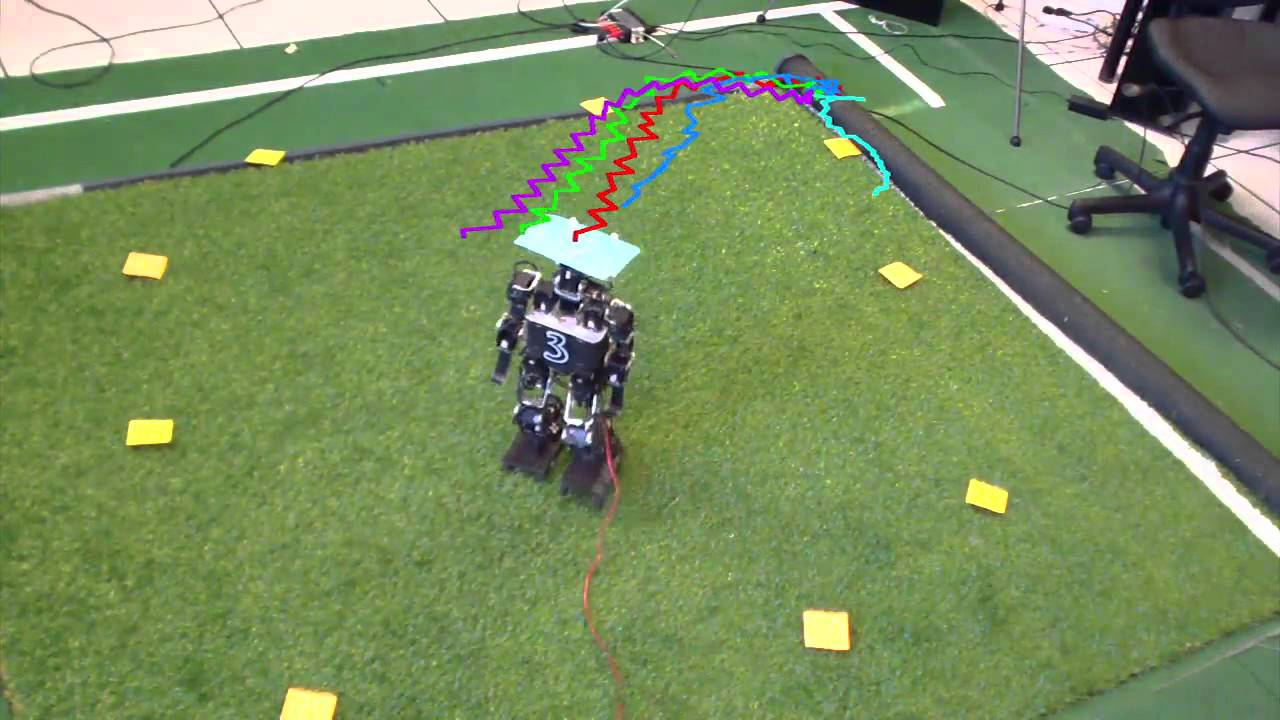
\includegraphics[width=0.8\linewidth]{../media/mocap_setup2.jpg}
        \caption{\label{fig:mocap_setup} Installation du système de capture de 
            mouvement (\textit{Motion Capture}) utilisée pour la mesure de la 
            pose du robot au cours de son déplacement. 
            Six caméras infrarouges sont disposées afin de couvrir la zone de capture.
            Un chapeau de plusieurs réflecteurs infrarouges est fixé sur la
            tête du robot.
            La zone de capture effective dans laquelle un nombre suffisent de marqueurs 
            sont toujours observés par au moins deux caméras ne fait que environ
            $1.5$~m\textsuperscript{2} (matérialisée par les marques au sol).
        }
    \end{center}
\end{figure}

La méthode proposée nécessite la mesure de la pose du robot
en permanence pendant son déplacement afin d'obtenir à chaque
pas la translation et la rotation du buste du robot dans le repère du monde.
Nous avons ici recours au système de capture de mouvement (\textit{Motion Capture} ou \textit{Mocap})
commercial \textit{OptiTrack}\footnote{Caméras OptiTrack Flex 13, 
\url{http://optitrack.com/products/flex-13/} et logiciel Motive, 
\url{http://optitrack.com/products/motive/}}.
Ce système se compose de six caméras hautes fréquences ($120$~Hz) à la fois recevant 
et émettant de la lumière infrarouge. 
La lumière infrarouge émise est reflétée par de petits
marqueurs placés sur le robot puis reçue par les caméras.
Les caméras sont disposées de sorte à couvrir avec un maximum de recouvrement
la zone de capture. Les marqueurs doivent être vus par au minimum deux caméras
à tout instant.
Enfin, un logiciel propriétaire analyse les images des six caméras et reconstruit
la position et l'orientation des marqueurs dans le repère du monde.
Ce repère est défini lors d'une phase préalable de calibration nécessitant environs
une quinzaine de minutes afin de calculer les positions relatives de toutes 
les caméras entres elles.
Ce système de détection permet à une fréquence de $100$~Hz de mesurer la position
et l'orientation d'un objet auquel est attaché un ensemble de marqueurs avec une
précision de l'ordre du millimètre.
La figure \ref{fig:mocap_setup} expose notre installation expérimentale.\\

Les principaux avantages de ce système de capture sont sa grande précision et
sa fréquence de mesure. Ils sont indispensables à cette technique de calibration.
Néanmoins, plusieurs facteurs limitent l'utilisation d'un tel système :
\begin{itemize}
    \item Le système est lourd à mettre en place. 
        Il nécessite plusieurs trépied et un ordinateur 
        possédant une puissance de calcul importante.
        L'installation n'est pas facilement déployable 
        dans un contexte opérationnel tel qu'un terrain de RoboCup.
    \item Malgré les six caméras, il est difficile d'obtenir une zone 
        de capture très étendue. Le déplacement du robot est alors 
        fortement contraint ce qui tend à générer des biais dans
        l'apprentissage et l'évaluation de l'odométrie précisés plus loin. 
        En effet, le robot effectue dans sa petite zone de nombreux 
        allers et retours exactement comme le remarque \cite{antonelli_calibration_2005}.
    \item Selon le placement des caméras ainsi que des conditions lumineuses 
        (et notamment la lumière naturelle), le suivi des marqueurs est 
        parfois peu robuste.
    \item Enfin, un soin particulier doit être porté à la configuration de l'objet
        reconstitué virtuellement défini par les marqueurs et dont la pose est suivi par le logiciel.
        En effet, il est crucial que la position et l'orientation de référence pour 
        le système soit bien bien aligné avec l'axe avant $\vec{\bm{x}}$ du robot. 
        Cet ajustement ne pouvant être réalisé que manuellement.
\end{itemize}

\subsection{Détail de l'architecture proposée}

\subsubsection{Protocole d'enregistrement des données}

L'enregistrement de données expérimentales est réalisé
sur le petit robot humanoïde de type Sigmaban. 
Plus précisément, il s'agit du robot numéro 3 Django équipé 
de moteurs Dynamixel RX (à potentiomètre) d'une précision angulaire 
maximum de $0.3$~degrés.
Le générateur de marche \textit{IKWalk} détaillé à la section 
\ref{sec:walk} est utilisé pour contrôler le robot.
Selon les cas, le processus de stabilisation utilisant
les capteurs de pression peut être ou non activé.
De plus, la surface au sol est soit de la moquette plate moyennement lisse,
soit de l'herbe artificielle dont les brins synthétiques 
ont une longueur de $3$~cm.

Le processus d'enregistrement des données est fortement contraint 
par le système de capture externe de mouvement.
Le système est tout d'abord installé, calibré et la zone effective
de mesure dans laquelle les marqueurs sont suffisamment visibles par 
les caméras est délimitée au sol.
Dans la zone de capture, le robot est piloté manuellement à la 
manette. La manette permet de contrôler à l'aide de deux joysticks
directement les trois paramètres dynamiques des ordres de la marche :
la translation avant arrière (\textit{stepGain}), latérale (\textit{lateralGain}) 
et la rotation (\textit{turnGain}) espérées à chaque pas.

Le robot doit pendant l'enregistrement des données éviter à tout prix
de sortir de la zone de capture. De plus, un maximum d'exploration dans
les ordres de la marche doit également être assuré. 
Enfin le robot ne doit pas se déstabiliser et tomber. 
D'autant plus lorsque le processus de stabilisation est désactivé.
Pour cette dernière raison, le pilotage manuel est préféré à un contrôle automatique
qui aurait pu améliorer la diversité des ordres en suivant un processus aléatoire
de Wiener (mouvement brownien).
Le pilotage de la marche suit donc les caractéristiques suivantes :
\begin{itemize}
    \item Des bornes minimales et maximales sont fixées aux trois 
        ordres de la marche afin de garantir un déplacement relativement stable.
    \item Manuellement, l'espace tridimensionnel des ordres est exploré en essayant
        de mélanger le plus possible les trois dimensions. Marche avant et arrière,
        pas latéraux et rotation simultané. 
        Plus généralement, des déplacements typiques des matchs de football robotiques
        (contournement de la balle, approche, ...) sont générés.
    \item Les bordures de la zone sont de capture sont évitées. 
        En pratique, la trajectoire du robot est amenée à faire de nombreux allers et retours
        ainsi que de nombreuses boucles. Même avec des limites de vitesses conservatives, 
        il ne faut qu'entre $10$ et $15$ secondes au robot pour traverser le diamètre de 
        la zone de capture.
    \item En observant continuellement la dynamique du robot, le pilotage \og expert \fg
        permet d'assurer que le robot ne tombe pas. Il est facile à voir (mais difficile à
        détecter automatiquement) quand le robot entre dans des oscillations parasites menant
        à sa déstabilisation. Une forte réduction des ordres de la marche permet généralement 
        de ramener la stabilité du système.
        Plus généralement, le pilotage à la manette contrôle finement les variations d'ordres 
        en fonction de l'état du robot. Il tend à limiter les grandes variations 
        d'ordres quand de fortes commandes sont mélangées. Par exemple, le robot est en effet 
        bien moins stable quand il subit une forte rotation en même temps qu'un fort déplacement latéral 
        et d'une marche arrière.
\end{itemize}

La longueur typique des enregistrements est de l'ordre de cinq minutes.
Il arrive néanmoins que durant ces séquences, le suivi des marqueurs soit perdu
pendant quelques secondes. 
Les points en question sont alors exclus automatiquement des données d'apprentissage.
Durant ces enregistrements, il est assuré que la marche du robot (les oscillations des pas)
ne s'arrête pas et que de plus, le robot ne tombe pas (même s'il peut temporairement
se trouver déstabilisé).

\subsubsection{Description de l'architecture}

\begin{figure}[htb]
    \begin{center}
        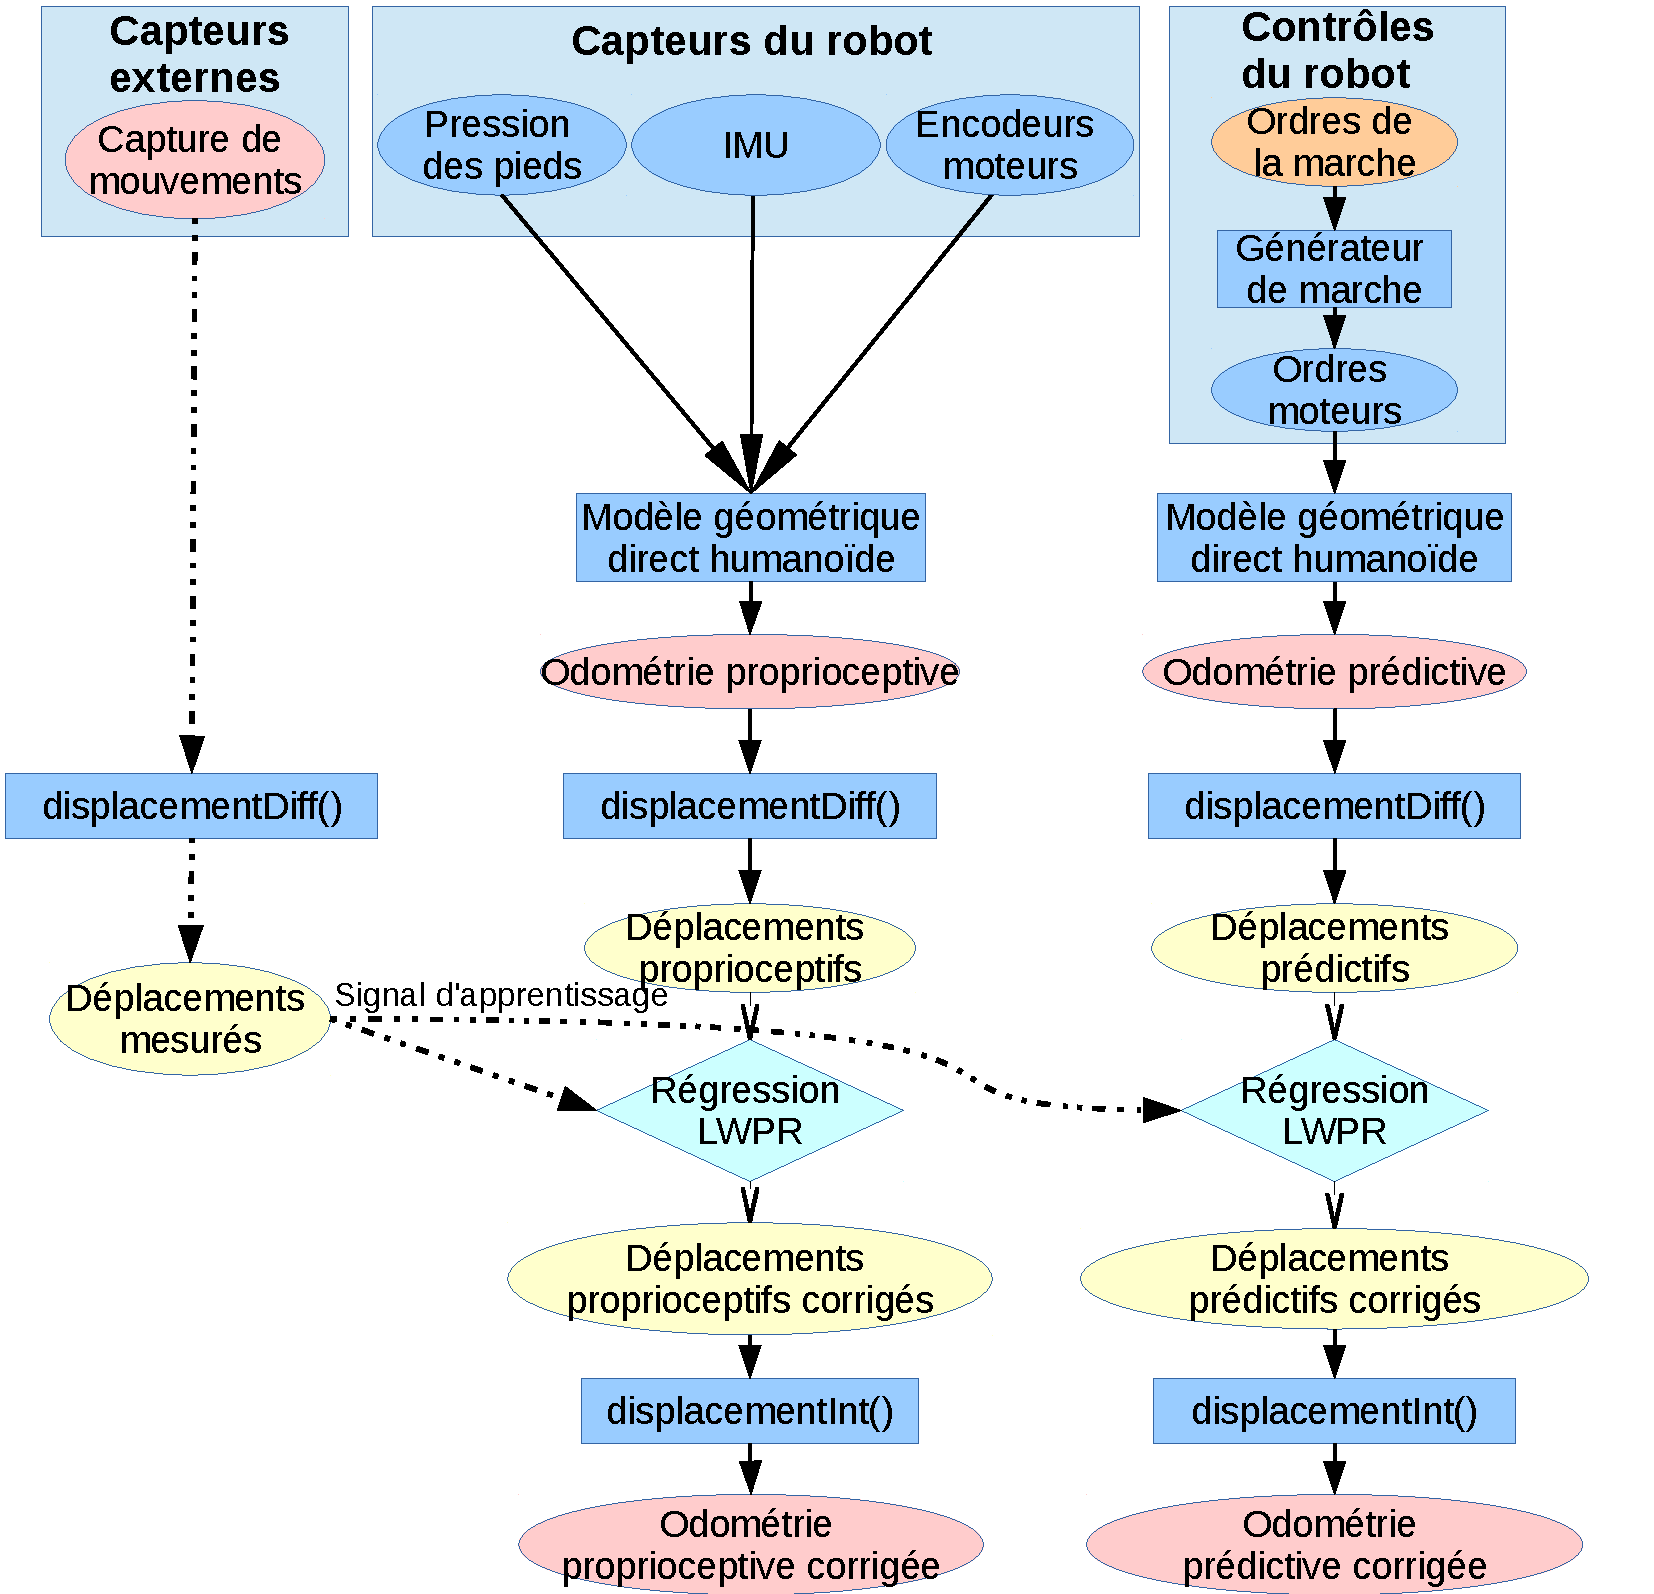
\includegraphics[type=pdf,ext=.pdf,read=.pdf,width=1.0\linewidth]{../schema/architecture}
        \caption{\label{fig:architecture_lwpr} 
            Architecture globale du système.
            Les ellipses représentent des valeurs et les
            rectangles représentent des fonctions abstraites.
            Les quatre odométries calculées (en rouge) sont comparées
            à la position réelle du robot mesurée par le système 
            de capture de mouvement.
        }
    \end{center}
\end{figure}

L'architecture de la méthode proposée est schématisée par la figure \ref{fig:architecture_lwpr}.
Pour rappel, ces travaux portent à la fois sur l'odométrie proprioceptive estimée pendant
le déplacement du robot au travers de ses capteurs ainsi que sur l'odométrie prédictive
(modèle de déplacement) à partir d'une séquence d'ordres de la marche.
Pendant la phase d'utilisation (ou d'exploitation) du système, son
fonctionnement est le suivant :\\

Lorsque le robot se déplace, la mesure de ses capteurs proprioceptifs 
(capteurs de pression, IMU et encodeurs) permet d'en déduire son état géométrique
(voir section \ref{sec:estimation_etat}) au travers du modèle géométrique direct.
En estimant le pied de support courant, la pose du robot peut alors être intégrée 
au cours du temps (sections \ref{sec:def_odometry} et \ref{sec:odometry_pressure}).
On obtient alors l'estimation de l'odométrie non corrigée dans le repère du monde.
Le but est alors d'appliquer une correction au déplacement estimé
afin de compenser les erreurs systématiques introduites par les glissements déterministes et
les erreurs de modélisations géométriques (torsion des pièces).

À chaque changement de pied de support, le déplacement relatif du buste du robot
entre deux pas est calculé en se basant 
sur la fonction $\mathsf{displacementDiff}()$\footnote{En pratique, le calcul 
des déplacements relatifs du robot est redondant avec l'intégration de l'odométrie 
réalisée au sein du modèle géométrique. 
La position est ici intégrée puis re-différentiée. 
Cette présentation des choses est choisie pour d'une part, 
la similarité de traitement entre l'odométrie estimée et la pose directement 
mesurée par le système de capture de mouvements. 
D'autre part, ceci permet d'abstraire la manière dont l'odométrie est effectivement estimée. 
Le principe général de la méthode pouvant s'appliquer à d'autres 
systèmes que les robots humanoïdes.}.
On obtient le déplacement proprioceptif entre deux pas du robot sous
la forme d'un vecteur tridimensionnel.
Ce vecteur est alors mis à jour au travers d'un appel au modèle de correction
appris par LWPR afin de rendre ce déplacement plus proche du déplacement réel du robot.
Enfin, ces déplacements relatifs sont ré-intégrés à l'aide de la fonction 
$\mathsf{displacementInt}()$ pour chaque changement de pied de support.
Le résultat de cette intégration est une odométrie estimée à partir 
des capteurs puis corrigée par le modèle LWPR.\\

Pour l'odométrie prédictive, le procédé est similaire.
À partir d'une séquence d'ordres, la simulation du générateur de marche 
calcule la séquence d'ordres moteurs associée.
Le modèle géométrique direct travail alors sur les positions désirées des moteurs.
Sans autre information disponible, le pied le plus bas dans le repère du monde est à tout instant
considéré comme pied de support. De plus, ce dernier est fixé plat par rapport au sol.
On obtient ainsi par intégration une odométrie prédictive et non corrigée.
La suite du traitement est identique au cas de l'odométrie en ligne.
À l'exception que le modèle de correction LWPR utilisé est bien celui du modèle de déplacement.
Les erreurs à corriger sont alors bien plus nombreuses puisqu'il faut capturer
toute la dynamique du système mécanique et les erreurs d'asservissement des moteurs.

L'intérêt de cette simulation géométrique du générateur de marche est de ne pas poser 
d'a priori sur les contrôles du mouvement. 
Typiquement, nous ne supposons pas que les ordres de la marche définissent 
directement le déplacement du buste du robot à chaque pas.
Mais si cette propriété est vérifiée, une optimisation du temps 
de calcul est alors possible.\\

Après l'enregistrement des données expérimentales, l'apprentissage se fait hors ligne.
De la même manière que pour l'odométrie, la pose du robot mesurée par le système
de capture de mouvement est découpée en déplacements relatifs à chaque changement de pied de support.
Ces déplacements relatifs sont considérés comme vérités terrain.
Ils sont utilisés comme référence lors de l'apprentissage puis comme point de comparaison lors de la validation.

\subsubsection{Apprentissages des fonctions de corrections\label{sec:odometry_lwpr_learning}}

Même si l'algorithme d'apprentissage de LWPR procède de manière
incrémental et peut s'exécuter en ligne, nous ne l'utilisons ici 
que hors ligne alors que toutes les données expérimentales sont disponibles.

On note de la manière suivante au moment du changement de pied de support $t$ respectivement, 
la pose du buste du robot mesurée par le système de capture de mouvement, 
l'odométrie proprioceptive (non corrigée) et l'odométrie prédictive (non corrigée) :
$$
\bm{p}_{t}^{\text{mocap}} = 
\begin{bmatrix}
    x_{t}^{\text{mocap}} \\
    y_{t}^{\text{mocap}} \\
    \theta_{t}^{\text{mocap}} \\
\end{bmatrix}
\in
\mathbb{R}^2 \times ]-\pi, \pi]
$$
$$
\bm{p}_{t}^{\text{read}}, \bm{p}_{t}^{\text{goal}}
\in
\mathbb{R}^2 \times ]-\pi, \pi]
$$

Les déplacements relatifs du buste du robot entre deux changements
de pied de support $t-1$ et $t$ successifs sont calculés :

$$
\Delta \bm{p}_{t}^{\text{mocap}} = 
\mathsf{displacementDiff}\big(\bm{p}_{t-1}^{\text{mocap}}, \bm{p}_{t}^{\text{mocap}}\big)
$$

De même pour $\Delta \bm{p}_{t}^{\text{read}}$ et $\Delta \bm{p}_{t}^{\text{goal}}$.

L'objectif de l'apprentissage LWPR est de construire à partir des données expérimentales 
les deux fonctions de correction non linéaires suivantes.
Elles transforment les déplacements relatifs proprioceptifs ou prédictifs
par les déplacements réellement mesurés sur le robot.

$$
\Delta \bm{p}_{t}^{\text{read}} \longmapsto \Delta \bm{p}_{t}^{\text{mocap}}
$$
$$
\Delta \bm{p}_{t}^{\text{goal}} \longmapsto \Delta \bm{p}_{t}^{\text{mocap}}
$$

Dans les détails, les déplacements du buste sont fortement dépendants du pied 
de support à cause des oscillations latérales de la marche. 
Il est ainsi nécessaire dans la régression de tenir compte du pied de support courant.
On note donc respectivement $s_{t}^{\text{read}}$ et $s_{t}^{\text{goal}} \in \{0, 1\}$,
les deux variables binaires indiquant lors du changement de pied de support $t$ si le
pied gauche ($1$) ou le pied droit ($0$) est le nouveau pied de support pour respectivement
les déplacements proprioceptifs et prédictifs.
De plus, il peut être important de prendre également en compte la dynamique du robot ; 
ses accélérations et ses décélérations.
Pour ce faire, on ajoute en entrée de la régression le précédant déplacement 
relatif au temps $t-1$.
Enfin, lorsque le robot marche et perd son équilibre, le processus de stabilisation
se basant sur les capteurs de pression stoppe temporairement le mouvement de marche.
La fréquence des oscillations de la marche est ainsi perturbée et la dynamique du robot affectée.
Pour prendre en compte ces évènements dans la correction de l'odométrie en ligne, 
les durées temporelles des deux pas successifs $l_{t-1}$ et $l_{t} \in \mathbb{R}_{+}$ sont utilisées.
On obtient alors le modèle suivant pour l'odométrie en ligne :

$$
\mathbb{R}^9 \longrightarrow \mathbb{R}^3
$$
$$
\big(\Delta \bm{p}_{t}^{\text{read}}, \Delta \bm{p}_{t-1}^{\text{read}}, s_{t}^{\text{read}}, l_{t}, l_{t-1}\big) 
\longmapsto \Delta \bm{p}_{t}^{\text{mocap}}
$$

Et le modèle suivant pour le modèle de déplacement.

$$
\mathbb{R}^7 \longrightarrow \mathbb{R}^3
$$
$$
\big(\Delta \bm{p}_{t}^{\text{goal}}, \Delta \bm{p}_{t-1}^{\text{goal}}, s_{t}^{\text{goal}}\big) 
\longmapsto \Delta \bm{p}_{t}^{\text{mocap}}
$$

Finalement, afin de simplifier le processus d'apprentissage, il est supposé que
les trois dimensions du déplacement mesuré $\Delta \bm{p}^{\text{mocap}}$ sont
indépendantes les unes des autres.
Cette approximation permet d'apprendre séparément avec LWPR six modèles distincts et univariés.

$$
\begin{cases}
\big(\Delta \bm{p}_{t}^{\text{read}}, \Delta \bm{p}_{t-1}^{\text{read}}, s_{t}^{\text{read}}, l_{t}, l_{t-1}\big) 
\longmapsto \Delta x_{t}^{\text{mocap}} \\
\big(\Delta \bm{p}_{t}^{\text{read}}, \Delta \bm{p}_{t-1}^{\text{read}}, s_{t}^{\text{read}}, l_{t}, l_{t-1}\big) 
\longmapsto \Delta y_{t}^{\text{mocap}} \\
\big(\Delta \bm{p}_{t}^{\text{read}}, \Delta \bm{p}_{t-1}^{\text{read}}, s_{t}^{\text{read}}, l_{t}, l_{t-1}\big) 
\longmapsto \Delta \theta_{t}^{\text{mocap}} \\
\end{cases}
$$
$$
\begin{cases}
\big(\Delta \bm{p}_{t}^{\text{goal}}, \Delta \bm{p}_{t-1}^{\text{goal}}, s_{t}^{\text{goal}}\big) 
\longmapsto \Delta x_{t}^{\text{mocap}} \\
\big(\Delta \bm{p}_{t}^{\text{goal}}, \Delta \bm{p}_{t-1}^{\text{goal}}, s_{t}^{\text{goal}}\big) 
\longmapsto \Delta y_{t}^{\text{mocap}} \\
\big(\Delta \bm{p}_{t}^{\text{goal}}, \Delta \bm{p}_{t-1}^{\text{goal}}, s_{t}^{\text{goal}}\big) 
\longmapsto \Delta \theta_{t}^{\text{mocap}} \\
\end{cases}
$$

\subsubsection{Optimisation des méta paramètres de LWPR}

\begin{table}[h]
    \centerfloat
    \small
    \begin{tabular}{|l|l|}
        \hline
        Méta paramètre & Valeur initiale \\
        \hline
        norm\_in & $0.05$ \\
        init\_alpha & $50.0$ \\
        meta\_rate & $250.0$ \\
        penalty & $10^{-6}$ \\
        init\_D & $1.0$ \\
        w\_gen & $0.1$ \\
        w\_prune & $0.9$ \\
        \hline
    \end{tabular}
    \caption{\label{tab:lwpr_meta_params}
        Liste des méta paramètres de LWPR et leurs valeurs initiales avant optimisation.
        La description de ses paramètres est détaillée par \cite{klanke_library_2008}.
    }
\end{table}

Au lieu d'ajuster manuellement tous les méta paramètres des 
six modèles LWPR, un algorithme d'optimisation en boite noire est utilisé 
(voir section \ref{sec:blackbox}).
La liste des paramètres et leurs valeurs initiales sont détaillées 
dans le tableau \ref{tab:lwpr_meta_params}.
L'algorithme génétique CMA-ES, \textit{Covariance Matrix Adaptation Evolution Strategy} ne 
demande pas de connaitre le gradient de la fonction à minimiser
(voir références et description de l'algorithme à la section \ref{sec:blackbox}).
Pour chacun des quatre contextes étudiés et chacun des six modèles LWPR, 
une phase d'optimisation préalable ajuste les méta paramètres en minimisant 
la fonction de récompense suivante :
\begin{itemize}
    \item Le modèle LWPR est initialisé avec le jeu de méta paramètres courant à évaluer.
    \item Le modèle apprend la correction des déplacements élémentaires 
        à partir d'un enregistrement expérimental.
    \item Un deuxième enregistrement est utilisé pour calculer l'erreur quadratique 
        moyenne (\textit{MSE}) de prédiction avec les déplacement réellement 
        mesurés par le système de capture de mouvement.
\end{itemize}
Au bout de $500$ itérations, les méta paramètres utilisés sont ceux minimisant sur l'ensemble de
validation l'erreur quadratique moyenne de prédiction.

\subsection{Expérimentation sur le robot Sigmaban et résultats}

Une vidéo résumant ces expérimentations peut être trouvée 
à l'adresse suivante :
\url{https://youtu.be/9HT33KMtfLw}

\subsubsection{Correction du délai de l'IMU}

\begin{figure}[htb]
    \centerfloat
    \begin{subfigure}{0.4\paperwidth}
        \centering
        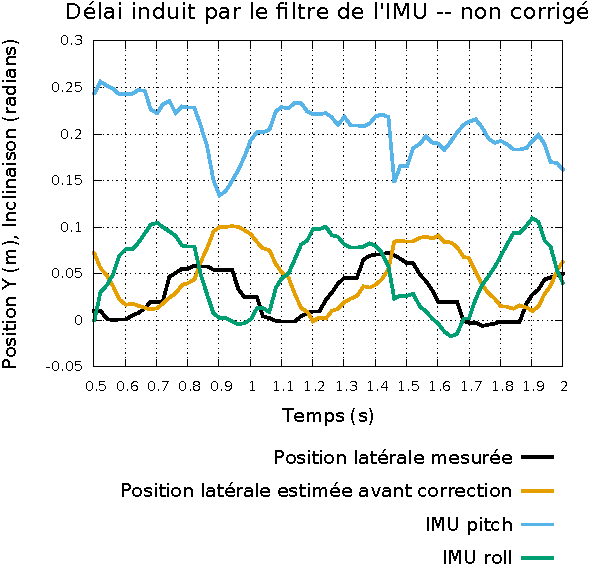
\includegraphics[type=pdf,ext=.pdf,read=.pdf,width=1.0\linewidth]{../plot/OdometryLWPR/grass_open_delay_imu_uncorrected}
    \end{subfigure}
    \begin{subfigure}{0.4\paperwidth}
        \centering
        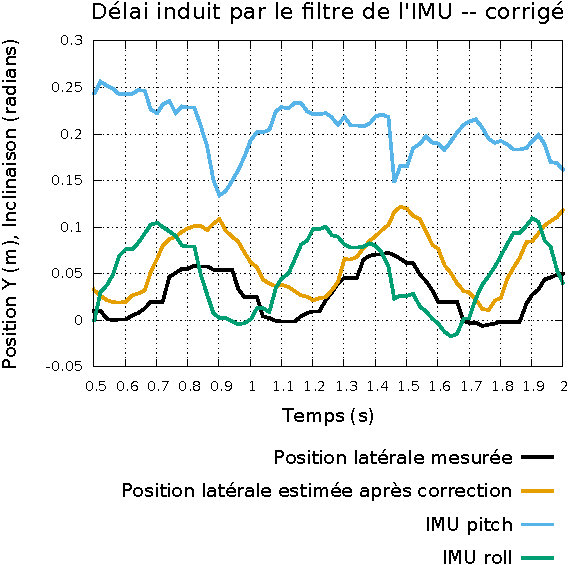
\includegraphics[type=pdf,ext=.pdf,read=.pdf,width=1.0\linewidth]{../plot/OdometryLWPR/grass_open_delay_imu_corrected}
    \end{subfigure}
    \caption{\label{fig:odometry_lwpr_imu_delay} 
        Illustration du délai introduit par le filtrage de la centrale inertielle et de sa correction. 
        Sans correction (à gauche), on observe un retard de la position latérale proprioceptive 
        du robot par rapport à la mesure externe.
        Les inclinaisons en tangage et en roulis fournis par l'IMU sont utilisés avec un décalage 
        de $160$~ms dans le futur afin de corriger (à droite) l'estimation de l'état du robot.
    }
\end{figure}

Les premières mesures expérimentales mettent en lumière un problème 
de délai non encore abordé jusqu'ici.
Pour rappel, la section \ref{sec:estimation_etat} décrit le filtrage de la centrale
inertielle estimant l'inclinaison du buste du robot par rapport à la verticale.
Or ce filtrage induit naturellement un délai qui s'avère en pratique impossible de négliger.
La figure \ref{fig:odometry_lwpr_imu_delay} sur le graphique de gauche montre en effet
que sans correction, on observe un important décalage temporel entre la mesure 
externe de la position latérale du robot et son estimation au travers de l'intégration 
du modèle géométrique direct. 
Ce retard de l'estimation sur la mesure est particulièrement visible 
sur les oscillations latérales du robot pendant le mouvement de marche.
Comme le montre le graphique, ce décalage provient bien du retard de l'inclinaison
en roulis (\textit{roll}) provoqué par le filtre de l'IMU.
Sans correction, les déplacements latéraux proprioceptifs sont
même en opposition de phase par rapport à la mesure externe.

Lors de l'estimation de l'état géométrique du robot à partir des capteurs, 
une correction temporelle de $160$~ms est appliquée.
Plus précisément, les valeurs de l'inclinaison du buste du robot fournies par 
le filtre (\textit{pitch} et \text{roll}) sont lues depuis les enregistrements 
avec une avance dans le futur.
L'estimation résultante de la position latérale du robot après correction 
est dépeinte à la droite de la figure \ref{fig:odometry_lwpr_imu_delay}.\\

À noter que les remarques détaillées dans cette section ne se concentrent 
que sur la plateforme robotique Sigmaban dans sa version 2015.
En effet en 2015, le filtre de l'IMU s'exécutait directement à bord d'un petit
microcontrôleur embarqué \textit{ATmega} associé à la centrale inertielle.
Dans les versions ultérieures, une puce rassemblant les capteurs seuls 
sans post-traitement a été préférée et le filtrage s'exécute maintenant 
à bord de l'ordinateur principal.
Ce déport permet une plus grande flexibilité dans le réglage et l'adaptation du filtre.
Néanmoins, le problème de fond persiste et un traitement similaire à celui présenté ici 
a été intégré de manière plus pérenne à l'architecture logiciel de \textit{RhobanServer}.
Un autre intérêt au déport du filtrage est que le délai observé et corrigé 
est alors plutôt de l'ordre de $20$~ms, 
soit beaucoup moins que précédemment\footnote{Nous n'avons pas entrepris d'expliquer plus avant 
le délai très important introduit par le filtrage à bord du microcontrôleur embarqué. 
Peut être sa très faible puissance de calcul flottante limite-t-elle
la fréquence à laquelle le filtre s'exécutait réellement.}.

\subsubsection{Jeux de données}

\begin{table}[h]
    \centerfloat
    \small
    \begin{tabular}{|l|l|l|p{2cm}|l|p{2.2cm}|p{2.2cm}|}
        \hline
        Surface & Marche & N° & Nombre de points & Durée (s) & Nombre de pas simulés & Nombre de pas mesurés \\
        \hline
        Herbe & Ouverte & 1 & 17929 & 358 & 670 & 664 \\
        Herbe & Ouverte & 2 & 19947 & 398 & 757 & 727 \\
        Herbe & Ouverte & 3 & 26322 & 526 & 1062 & 1061 \\
        Herbe & Ouverte & 4 & 21688 & 433 & 910 & 863 \\
        \hline
        Herbe & Fermée & 1 & 16693 & 333 & 406 & 409 \\
        Herbe & Fermée & 2 & 17229 & 344 & 511 & 535 \\
        Herbe & Fermée & 3 & 23557 & 471 & 655 & 689 \\
        Herbe & Fermée & 4 & 21017 & 420 & 616 & 626 \\
        Herbe & Fermée & 5 & 18357 & 367 & 501 & 477 \\
        \hline
        Moquette & Ouverte & 1 & 16228 & 324 & 609 & 571 \\
        Moquette & Ouverte & 2 & 15831 & 316 & 650 & 577 \\
        Moquette & Ouverte & 3 & 19144 & 382 & 773 & 807 \\
        Moquette & Ouverte & 4 & 17492 & 349 & 685 & 691 \\
        Moquette & Ouverte & 5 & 16932 & 338 & 700 & 636 \\
        \hline
        Moquette & Fermée & 1 & 19094 & 381 & 571 & 731 \\
        Moquette & Fermée & 2 & 18346 & 366 & 471 & 506 \\
        Moquette & Fermée & 3 & 21598 & 432 & 546 & 583 \\
        \hline
    \end{tabular}
    \caption{\label{tab:odometry_logs}Liste des enregistrements expérimentaux 
        de l'odométrie sur Sigmaban (version 2015). 
        Le nombre de pas représente la taille des ensembles 
        d'apprentissage et de validation. 
    Les pas pendant lesquels le suivi de mouvement est perdu ne sont pas considérés.}
\end{table}

Quatre conditions expérimentales sont étudiées et comparées.
La surface au sol est soit du gazon artificiel, soit une simple moquette fine.
Le processus de stabilisation du mouvement de marche peux être activé ou non. 
La pose réelle du robot est mesurée par le système de capture de mouvement
et l'ensemble des capteurs ainsi que les ordres envoyés au mouvement de marche 
sont enregistrés à la fréquence de $50$~Hz\footnote{Plateforme Sigmaban 2015}.

L'ensemble des enregistrements réalisés dans les différents contextes 
sont listés dans le tableau \ref{tab:odometry_logs}.
Le tableau précise pour chaque enregistrement son contexte, le nombre total de 
points (correspondant à un horodatage) capturés, sa durée ainsi que 
le nombre de déplacements proprioceptifs et prédictifs exploitables 
entre deux changements de pieds de support.
À chaque enregistrement est également associé un numéro.
Ces numéros assignent aux enregistrements les rôles suivant :
\begin{itemize}
    \item \textbf{Enregistrement n°1 : }Ensemble d'apprentissage pour l'optimisation des méta paramètres de LWPR.
    \item \textbf{Enregistrement n°2 : }Ensemble de validation pour l'optimisation des méta paramètres de LWPR.
    \item \textbf{Enregistrement n°3 : }Ensemble d'apprentissage pour la phase d'évaluation.
    \item Les autres enregistrements disponibles sont utilisés comme ensemble de validation 
        pour l'évaluation de la méthode.
\end{itemize}
Dans le cas de l'odométrie sur moquette et en boucle fermée, l'enregistrement numéro 2 
est utilisé à la fois pour valider l'optimisation des méta paramètres et pour 
l'évaluation de la précision de la méthode.

\begin{figure}[htbp]
    \centerfloat
    \begin{subfigure}{0.22\paperwidth}
        \centering
        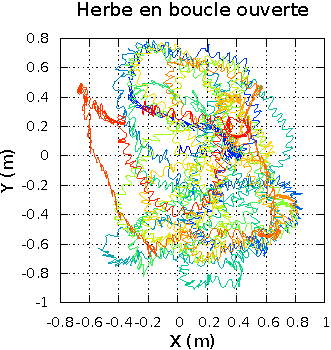
\includegraphics[type=pdf,ext=.pdf,read=.pdf,width=1.0\linewidth]{../plot/OdometryLWPR/grass_open_learn_log_complete_traj}
    \end{subfigure}
    \begin{subfigure}{0.22\paperwidth}
        \centering
        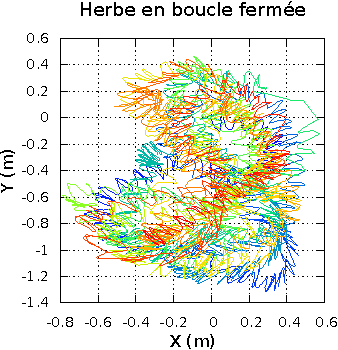
\includegraphics[type=pdf,ext=.pdf,read=.pdf,width=1.0\linewidth]{../plot/OdometryLWPR/grass_close_learn_log_complete_traj}
    \end{subfigure}
    \begin{subfigure}{0.22\paperwidth}
        \centering
        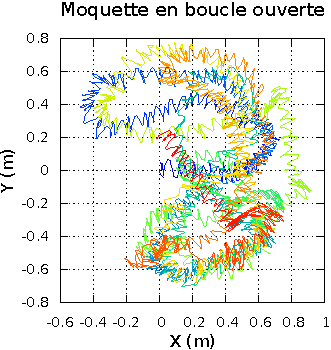
\includegraphics[type=pdf,ext=.pdf,read=.pdf,width=1.0\linewidth]{../plot/OdometryLWPR/carpet_open_learn_log_complete_traj}
    \end{subfigure}
    \begin{subfigure}{0.22\paperwidth}
        \centering
        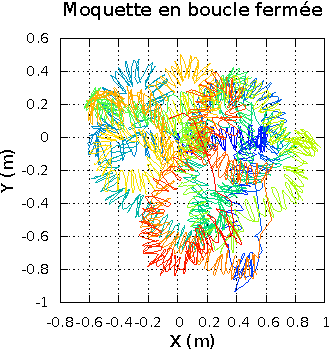
\includegraphics[type=pdf,ext=.pdf,read=.pdf,width=1.0\linewidth]{../plot/OdometryLWPR/carpet_close_learn_log_complete_traj}
    \end{subfigure}
    \newline
    \begin{subfigure}{0.22\paperwidth}
        \centering
        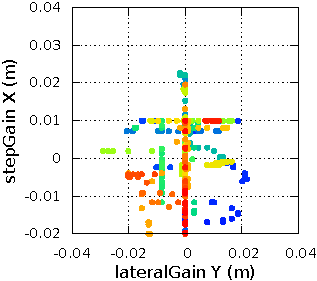
\includegraphics[type=pdf,ext=.pdf,read=.pdf,width=1.0\linewidth]{../plot/OdometryLWPR/grass_open_learn_log_walk_orders}
    \end{subfigure}
    \begin{subfigure}{0.22\paperwidth}
        \centering
        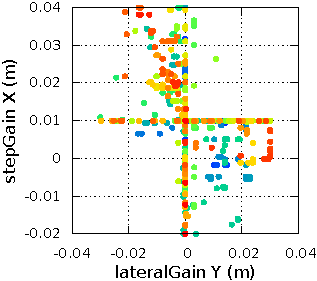
\includegraphics[type=pdf,ext=.pdf,read=.pdf,width=1.0\linewidth]{../plot/OdometryLWPR/grass_close_learn_log_walk_orders}
    \end{subfigure}
    \begin{subfigure}{0.22\paperwidth}
        \centering
        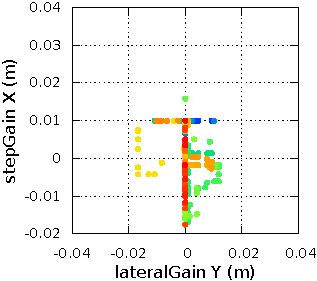
\includegraphics[type=pdf,ext=.pdf,read=.pdf,width=1.0\linewidth]{../plot/OdometryLWPR/carpet_open_learn_log_walk_orders}
    \end{subfigure}
    \begin{subfigure}{0.22\paperwidth}
        \centering
        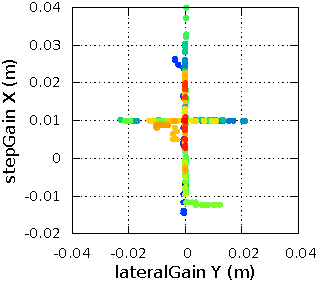
\includegraphics[type=pdf,ext=.pdf,read=.pdf,width=1.0\linewidth]{../plot/OdometryLWPR/carpet_close_learn_log_walk_orders}
    \end{subfigure}
    \caption{\label{fig:odometry_lwpr_logs} 
        La première ligne montre la position mesurée au cours du temps du robot 
        sur le plan du sol par le système de capture de mouvement.
        Les quatre enregistrements d'apprentissage complets (enregistrements numéro 3)
        sont représentés pour chacune des conditions comparées.
        On observe les multiples allers et retours du robot piloté manuellement.
        La deuxième ligne montre pour chaque contexte (en colonne) 
        l'espace d'action des ordres de la marche (paramètres dynamiques 
        envoyés au mouvement IKWalk) d'avance et de latéral.
        La dispersion des points montre l'exploration manuelle de l'espace des ordres.
        On remarque un fort regroupement sur les axes $X$ et $Y$ induit mécaniquement 
        par le joystick de la manette.
        La couleur représente l'évolution du temps du bleu au rouge.
    }
\end{figure}

La figure \ref{fig:odometry_lwpr_logs} présente pour chacun des quatre 
contextes étudiés l'enregistrement sur lequel est effectué l'apprentissage.
La position mesurée par le système de capture de mouvement sur l'enregistrement complet
ainsi que la projection des ordres de la marche dans sur le 
plan $(\Delta x, \Delta y)$ sont représentés.
L'étendue de zone de capture d'environ $1.5$~$m^2$ se devine (le centre du référentiel 
sur le sol est à chaque fois différent).
On y voit le robot faire de multiples boucles dans la zone de capture.

Pour les ordres de la marche, chaque point correspond à un ordre de déplacement 
entre deux changements de pied de support.
On observe alors que les points sont particulièrement regroupés sur les axes $X$ et $Y$.
Ceci semble provenir d'une caractéristique mécanique des joystick de la manette utilisée.
Pour améliorer l'ergonomie, la réponse du joystick n'est absolument pas linéaire mais
présente des effets de seuil à la fois aux alentours de la position neutre mais également 
aux alentours de la position maximal.
Malheureusement, cette caractéristique rend l'exploration manuelle de l'espace de
contrôle particulièrement malaisée.

En conséquence, la couverture de l'espace de contrôle est loin d'être idéale.
Il serait certainement profitable d'envisager un contrôle hybride mélangeant une exploration
plus aléatoire mais néanmoins dont la direction ou l'accélération serait guidée manuellement
afin de respecter les contraintes mentionnées dans la section \ref{sec:odometry_mocap}.

\subsubsection{Analyse des données}

\begin{figure}[htbp]
    \centerfloat
    \begin{subfigure}{0.22\paperwidth}
        \centering
        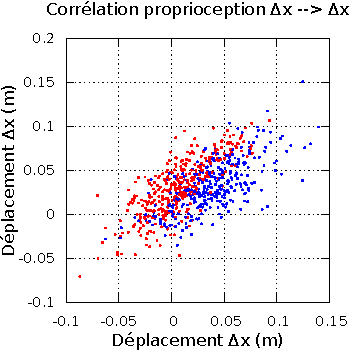
\includegraphics[type=pdf,ext=.pdf,read=.pdf,width=1.0\linewidth]{../plot/OdometryLWPR/grass_close_function_read_x_x}
    \end{subfigure}
    \begin{subfigure}{0.22\paperwidth}
        \centering
        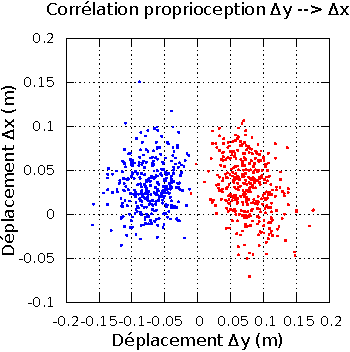
\includegraphics[type=pdf,ext=.pdf,read=.pdf,width=1.0\linewidth]{../plot/OdometryLWPR/grass_close_function_read_y_x}
    \end{subfigure}
    \begin{subfigure}{0.22\paperwidth}
        \centering
        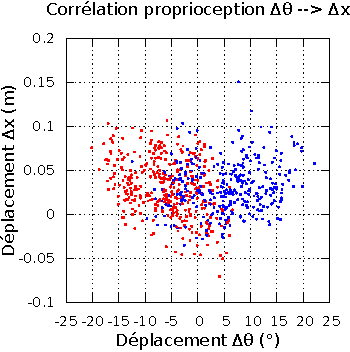
\includegraphics[type=pdf,ext=.pdf,read=.pdf,width=1.0\linewidth]{../plot/OdometryLWPR/grass_close_function_read_yaw_x}
    \end{subfigure}
    \begin{subfigure}{0.22\paperwidth}
        \centering
        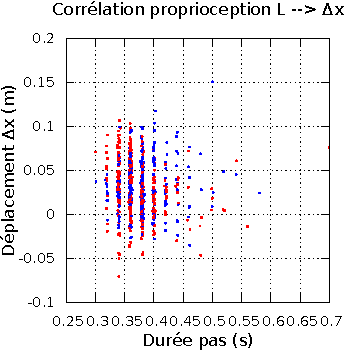
\includegraphics[type=pdf,ext=.pdf,read=.pdf,width=1.0\linewidth]{../plot/OdometryLWPR/grass_close_function_read_len_x}
    \end{subfigure}
    \vspace{0.2cm}
    \newline
    \begin{subfigure}{0.22\paperwidth}
        \centering
        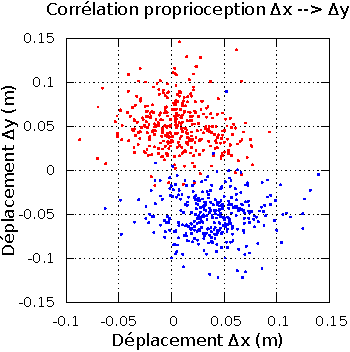
\includegraphics[type=pdf,ext=.pdf,read=.pdf,width=1.0\linewidth]{../plot/OdometryLWPR/grass_close_function_read_x_y}
    \end{subfigure}
    \begin{subfigure}{0.22\paperwidth}
        \centering
        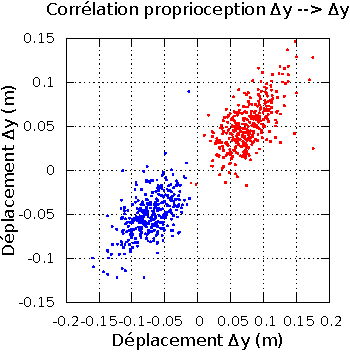
\includegraphics[type=pdf,ext=.pdf,read=.pdf,width=1.0\linewidth]{../plot/OdometryLWPR/grass_close_function_read_y_y}
    \end{subfigure}
    \begin{subfigure}{0.22\paperwidth}
        \centering
        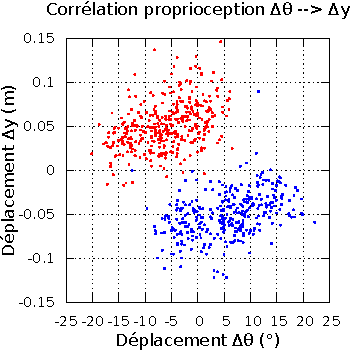
\includegraphics[type=pdf,ext=.pdf,read=.pdf,width=1.0\linewidth]{../plot/OdometryLWPR/grass_close_function_read_yaw_y}
    \end{subfigure}
    \begin{subfigure}{0.22\paperwidth}
        \centering
        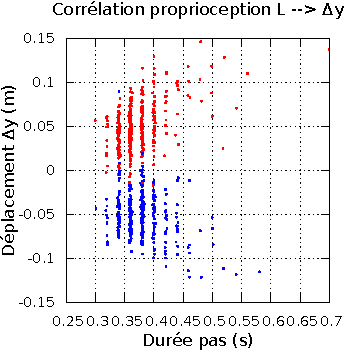
\includegraphics[type=pdf,ext=.pdf,read=.pdf,width=1.0\linewidth]{../plot/OdometryLWPR/grass_close_function_read_len_y}
    \end{subfigure}
    \vspace{0.2cm}
    \newline
    \begin{subfigure}{0.22\paperwidth}
        \centering
        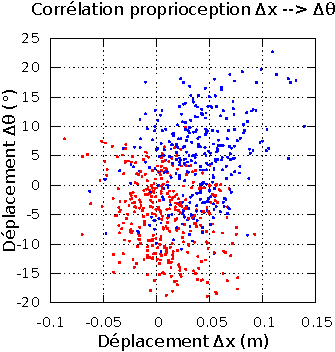
\includegraphics[type=pdf,ext=.pdf,read=.pdf,width=1.0\linewidth]{../plot/OdometryLWPR/grass_close_function_read_x_yaw}
    \end{subfigure}
    \begin{subfigure}{0.22\paperwidth}
        \centering
        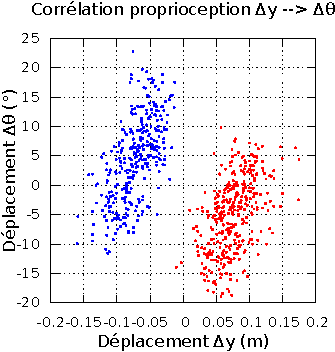
\includegraphics[type=pdf,ext=.pdf,read=.pdf,width=1.0\linewidth]{../plot/OdometryLWPR/grass_close_function_read_y_yaw}
    \end{subfigure}
    \begin{subfigure}{0.22\paperwidth}
        \centering
        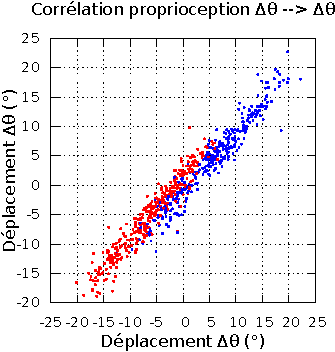
\includegraphics[type=pdf,ext=.pdf,read=.pdf,width=1.0\linewidth]{../plot/OdometryLWPR/grass_close_function_read_yaw_yaw}
    \end{subfigure}
    \begin{subfigure}{0.22\paperwidth}
        \centering
        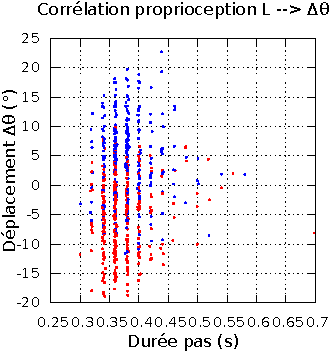
\includegraphics[type=pdf,ext=.pdf,read=.pdf,width=1.0\linewidth]{../plot/OdometryLWPR/grass_close_function_read_len_yaw}
    \end{subfigure}
    \caption{\label{fig:odometry_lwpr_function_read} 
        Détail des corrélations entre les déplacements proprioceptifs et les déplacements
        mesurés par le système de capture de mouvement.
        Les distances sont exprimées en mètres et les angles en degrés.
        Les trois composantes $(\Delta x, \Delta y, \Delta \theta)$ des déplacements mesurés sont présentées en ordonné
        alors que les trois composantes des déplacements de base ainsi que la durée des pas $L$ sont présentées en abscisse.
        Les points en bleu représentent les déplacements en phase de support droit et en rouge en phase de support gauche.
        Il s'agit des données issues de l'enregistrement numéro $3$ sur herbe artificielle en boucle fermée.
    }
\end{figure}

\begin{figure}[htbp]
    \centerfloat
    \begin{subfigure}{0.22\paperwidth}
        \centering
        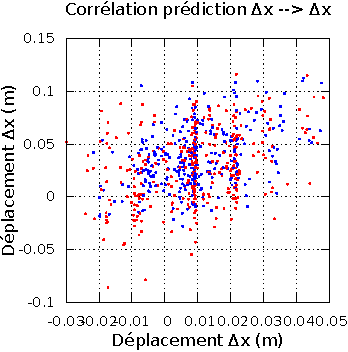
\includegraphics[type=pdf,ext=.pdf,read=.pdf,width=1.0\linewidth]{../plot/OdometryLWPR/grass_close_function_goal_x_x}
    \end{subfigure}
    \begin{subfigure}{0.22\paperwidth}
        \centering
        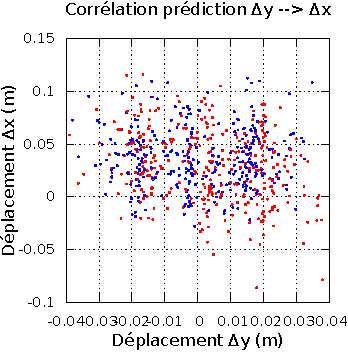
\includegraphics[type=pdf,ext=.pdf,read=.pdf,width=1.0\linewidth]{../plot/OdometryLWPR/grass_close_function_goal_y_x}
    \end{subfigure}
    \begin{subfigure}{0.22\paperwidth}
        \centering
        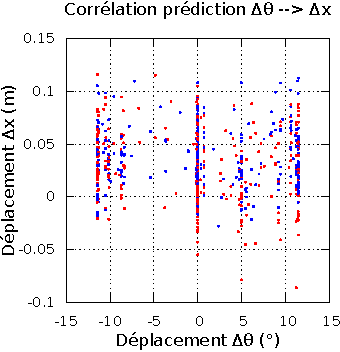
\includegraphics[type=pdf,ext=.pdf,read=.pdf,width=1.0\linewidth]{../plot/OdometryLWPR/grass_close_function_goal_yaw_x}
    \end{subfigure}
    \vspace{0.2cm}
    \newline
    \begin{subfigure}{0.22\paperwidth}
        \centering
        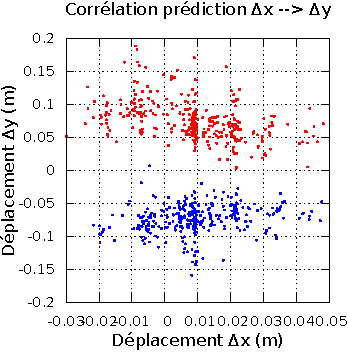
\includegraphics[type=pdf,ext=.pdf,read=.pdf,width=1.0\linewidth]{../plot/OdometryLWPR/grass_close_function_goal_x_y}
    \end{subfigure}
    \begin{subfigure}{0.22\paperwidth}
        \centering
        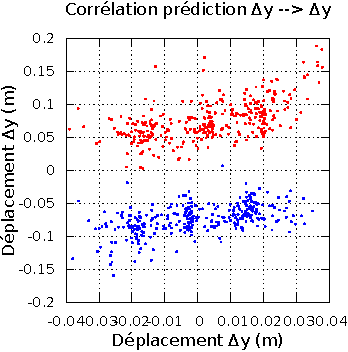
\includegraphics[type=pdf,ext=.pdf,read=.pdf,width=1.0\linewidth]{../plot/OdometryLWPR/grass_close_function_goal_y_y}
    \end{subfigure}
    \begin{subfigure}{0.22\paperwidth}
        \centering
        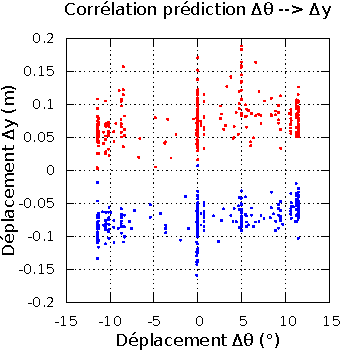
\includegraphics[type=pdf,ext=.pdf,read=.pdf,width=1.0\linewidth]{../plot/OdometryLWPR/grass_close_function_goal_yaw_y}
    \end{subfigure}
    \vspace{0.2cm}
    \newline
    \begin{subfigure}{0.22\paperwidth}
        \centering
        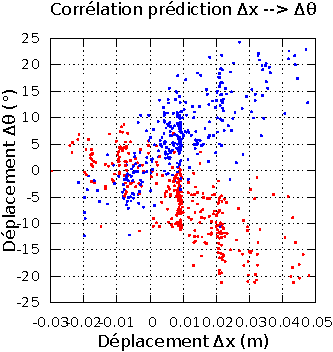
\includegraphics[type=pdf,ext=.pdf,read=.pdf,width=1.0\linewidth]{../plot/OdometryLWPR/grass_close_function_goal_x_yaw}
    \end{subfigure}
    \begin{subfigure}{0.22\paperwidth}
        \centering
        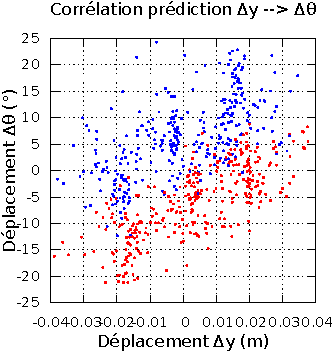
\includegraphics[type=pdf,ext=.pdf,read=.pdf,width=1.0\linewidth]{../plot/OdometryLWPR/grass_close_function_goal_y_yaw}
    \end{subfigure}
    \begin{subfigure}{0.22\paperwidth}
        \centering
        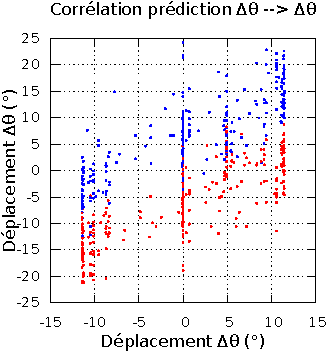
\includegraphics[type=pdf,ext=.pdf,read=.pdf,width=1.0\linewidth]{../plot/OdometryLWPR/grass_close_function_goal_yaw_yaw}
    \end{subfigure}
    \caption{\label{fig:odometry_lwpr_function_goal} 
        Détail des corrélations entre les déplacements prédictifs et les déplacements
        mesurés par le système de capture de mouvement.
        Les distances sont exprimées en mètres et les angles en degrés.
        Les trois composantes $(\Delta x, \Delta y, \Delta \theta)$ des déplacements mesurés sont présentées en ordonné
        alors que les trois composantes des déplacements prédicitfs sont présentées en abscisse.
        Les points en bleu représentent les déplacements en phase de support droit et en rouge en phase de support gauche.
        Il s'agit des données issues de l'enregistrement numéro $3$ sur herbe artificielle en boucle fermée.
    }
\end{figure}

Avant de détailler la phase d'apprentissage, les figures \ref{fig:odometry_lwpr_function_read} 
et \ref{fig:odometry_lwpr_function_goal} analysent la forme des fonctions de correction
des déplacements recherchés.
La projection des corrélations entre les déplacements de base et les déplacements mesurés 
par la capture de mouvement est représentée composante par composante.
La figure \ref{fig:odometry_lwpr_function_read} détaille les déplacements proprioceptifs, 
$\big(\Delta p_{t}^{\text{read}}, l_{t}\big) \longmapsto \Delta p_{t}^{\text{mocap}}$.
Tandis que la figure \ref{fig:odometry_lwpr_function_goal} fait de même 
avec les déplacements prédictifs, 
$\big(\Delta p_{t}^{\text{goal}}\big) \longmapsto \Delta p_{t}^{\text{mocap}}$.
A chaque fois, la couleur permet de séparer les points associés aux déplacements en phase 
de support gauche et en phase de support droit.

La première observation est que le bruit affectant les déplacements est très important.
La conjonction des défauts de lissage du générateur de marche \textit{IKWalk}, de la qualité 
du contrôle moteur, des chocs avec le sol et des jeux mécaniques rendent 
le système mécanique du robot sujet à de nombreuses perturbations non déterministes.

Néanmoins, une corrélation forte est bien visible sur les relations
directes : $\Delta x_{t} \mapsto \Delta x_{t}^{\text{mocap}}$, 
$\Delta y_{t} \mapsto \Delta y_{t}^{\text{mocap}}$ et 
$\Delta \theta_{t} \mapsto \Delta \theta_{t}^{\text{mocap}}$.
De plus comme attendu, cette relation est plus proche de l'identité avec 
les déplacements proprioceptifs que des déplacements prédictifs.
Les déplacement prédictifs tendent à grandement sous estimer les distances.
Ceci est dû aux erreurs de contrôle moteur. En réalité, la trajectoire des pieds du
robot dépasse la consigne en position à cause des effets inertiels non pris en compte
et les pas effectifs sont alors plus grands que prévus. 
On voit également l'importance de prendre en compte l'information du pied du support 
car les déplacements notamment latéraux sont opposés.

On observe ensuite que certaines relations croisées ont une influence également importante.
Par exemple, les rotations influencent nettement les translations latérales 
$\Delta y_{t} \mapsto \Delta \theta_{t}^{\text{mocap}}$ aussi bien sur les déplacements 
proprioceptifs que prédcitifs.

L'enregistrement sur lequel s'appuie ces graphiques est réalisé avec un mouvement
de marche en boucle fermée. 
Pendant l'enregistrement, le robot n'a pas délibérément été déstabilisé. 
Au contraire, le pilotage manuel a pris garde de limiter les accélérations pouvant mener 
aux perturbations de l'équilibre du robot.
En conséquence, les données récoltées ici ne sont pas vraiment suffisantes 
pour conclure sur l'influence de la longueur des pas même si une tendance semble se dessiner.
Cette tendance se remarque surtout sur les déplacements latéraux. 
C'est en effet sur les pas chassés que la stabilisation par les capteurs de pression 
est particulièrement importante pour améliorer la robustesse de la marche.

Enfin, même si la relation $\Delta \theta_{t}^{\text{read}} \mapsto \Delta x_{t}^{\text{mocap}}$ 
semble avoir une très légère tendance quadratique, les autres corrélations sont nettement linéaires.
Le bruit est en effet trop important pour capturer des relations plus fines.
En conclusion, l'utilisation de l'algorithme de régression non paramétrique ne parait pas
réellement nécessaire\footnote{Une étude qualitative préalable réalisée un an auparavant avait 
dans des conditions plus simples laissé croire à des relations plus complexes. 
Cette étude avait motivée le choix de la méthode LWPR. L'odométrie des robots est néanmoins 
très dépendante de la plateforme robotique et entre temps, le robot à subit de nombreuses évolutions.}.
Après analyse, un modèle paramétrique purement linéaire aurait certainement capturé
la plus grande part des corrélations constatées ici.

\subsubsection{Convergence de l'apprentissage et analyse}

\begin{figure}[htb] 
    \centerfloat
    \vspace{-0.5cm}
    %%%% Grass Open
    \begin{subfigure}{0.29\paperwidth}
        \centering
        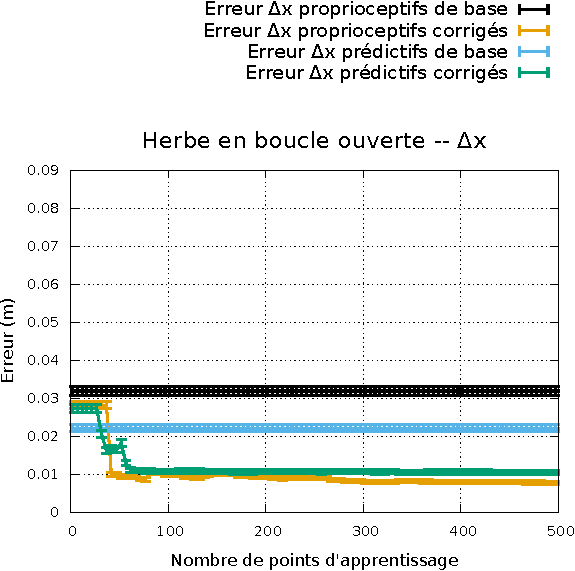
\includegraphics[type=pdf,ext=.pdf,read=.pdf,width=1.0\linewidth]{../plot/OdometryLWPR/grass_open_convergence_x}
    \end{subfigure}
    \begin{subfigure}{0.29\paperwidth}
        \centering
        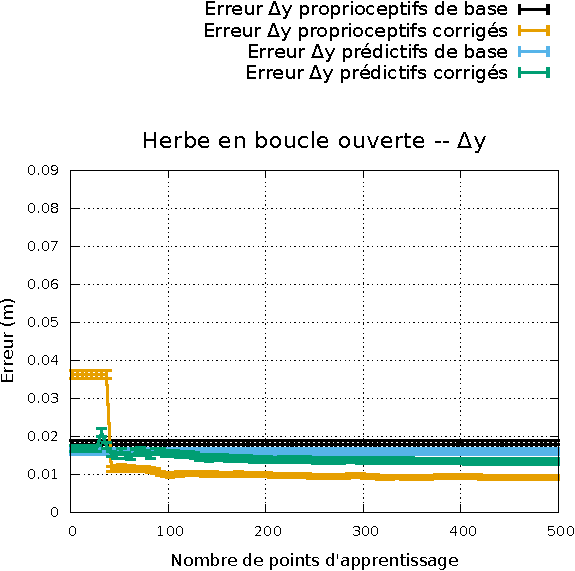
\includegraphics[type=pdf,ext=.pdf,read=.pdf,width=1.0\linewidth]{../plot/OdometryLWPR/grass_open_convergence_y}
    \end{subfigure}
    \begin{subfigure}{0.29\paperwidth}
        \centering
        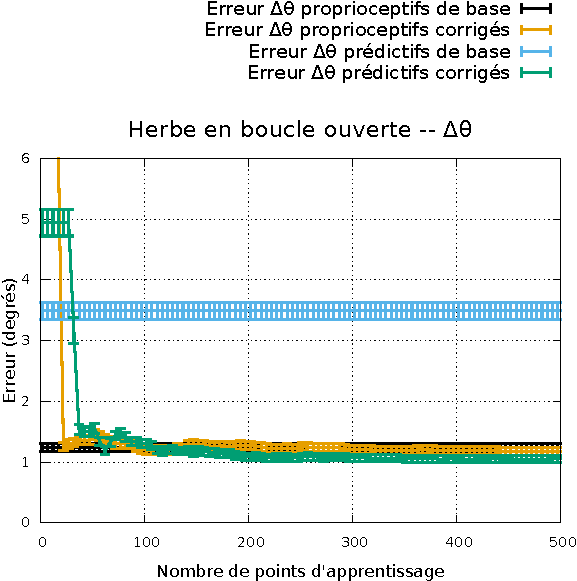
\includegraphics[type=pdf,ext=.pdf,read=.pdf,width=1.0\linewidth]{../plot/OdometryLWPR/grass_open_convergence_yaw}
    \end{subfigure}
    %%%% Grass Close
    \vspace{0.1cm}
    \newline
    \begin{subfigure}{0.29\paperwidth}
        \centering
        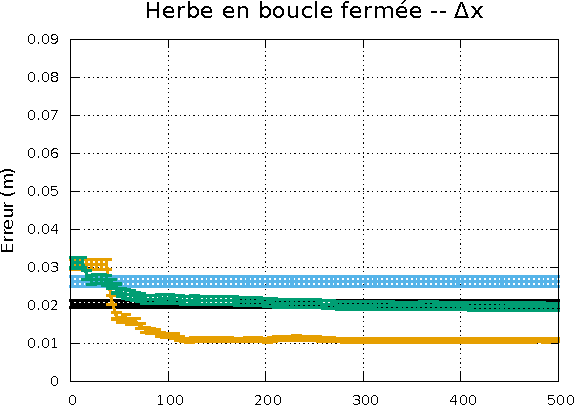
\includegraphics[type=pdf,ext=.pdf,read=.pdf,width=1.0\linewidth]{../plot/OdometryLWPR/grass_close_convergence_x}
    \end{subfigure}
    \begin{subfigure}{0.29\paperwidth}
        \centering
        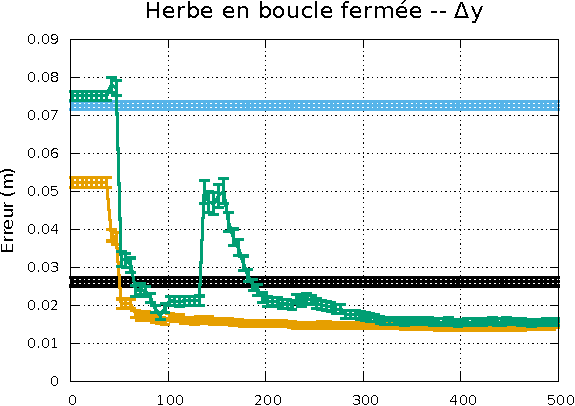
\includegraphics[type=pdf,ext=.pdf,read=.pdf,width=1.0\linewidth]{../plot/OdometryLWPR/grass_close_convergence_y}
    \end{subfigure}
    \begin{subfigure}{0.29\paperwidth}
        \centering
        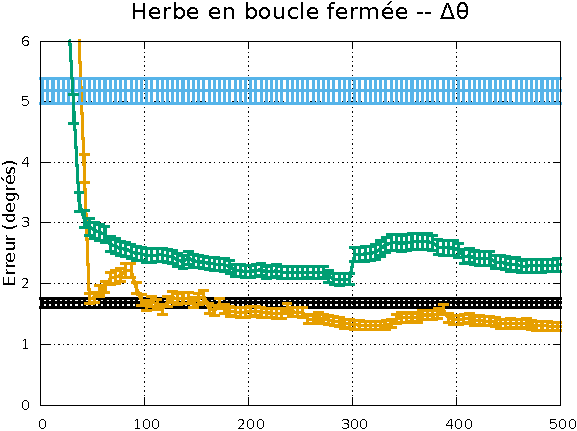
\includegraphics[type=pdf,ext=.pdf,read=.pdf,width=1.0\linewidth]{../plot/OdometryLWPR/grass_close_convergence_yaw}
    \end{subfigure}
    %%%% Carpet Open
    \vspace{0.1cm}
    \newline
    \begin{subfigure}{0.29\paperwidth}
        \centering
        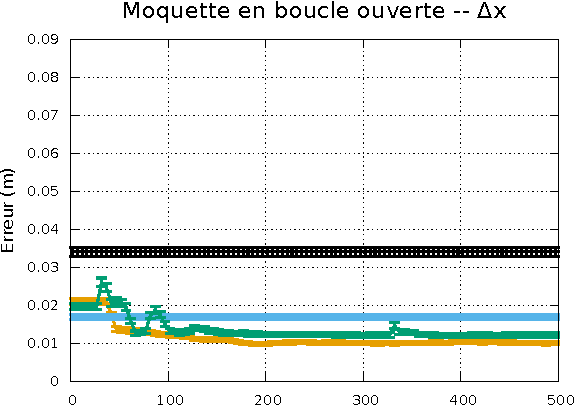
\includegraphics[type=pdf,ext=.pdf,read=.pdf,width=1.0\linewidth]{../plot/OdometryLWPR/carpet_open_convergence_x}
    \end{subfigure}
    \begin{subfigure}{0.29\paperwidth}
        \centering
        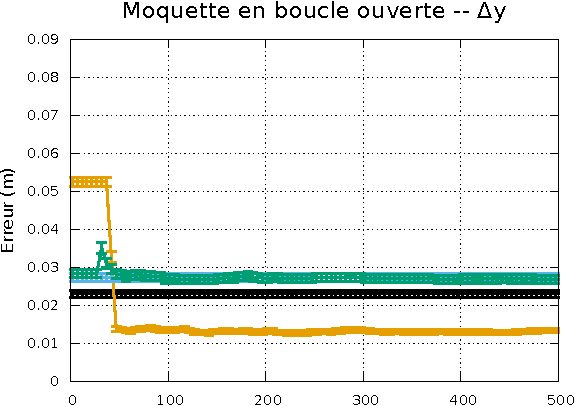
\includegraphics[type=pdf,ext=.pdf,read=.pdf,width=1.0\linewidth]{../plot/OdometryLWPR/carpet_open_convergence_y}
    \end{subfigure}
    \begin{subfigure}{0.29\paperwidth}
        \centering
        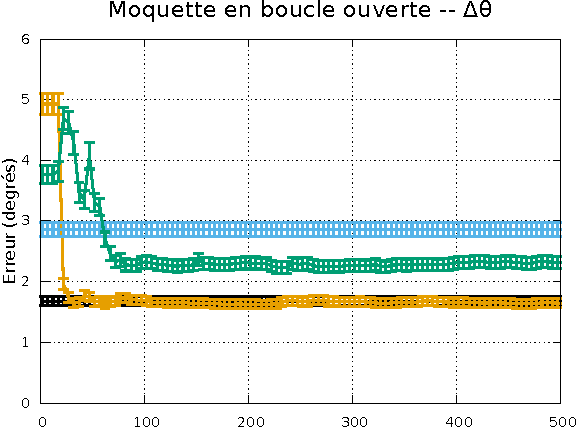
\includegraphics[type=pdf,ext=.pdf,read=.pdf,width=1.0\linewidth]{../plot/OdometryLWPR/carpet_open_convergence_yaw}
    \end{subfigure}
    %%%% Carpet Close
    \vspace{0.1cm}
    \newline
    \begin{subfigure}{0.29\paperwidth}
        \centering
        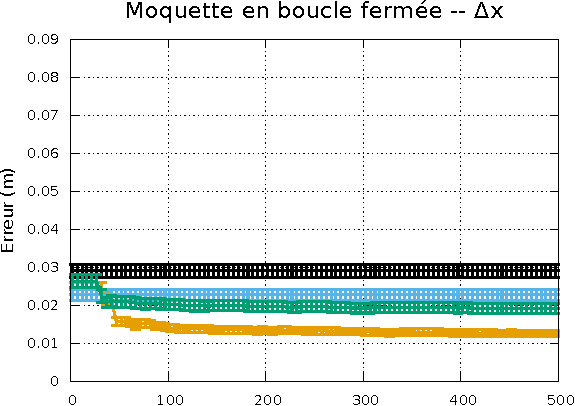
\includegraphics[type=pdf,ext=.pdf,read=.pdf,width=1.0\linewidth]{../plot/OdometryLWPR/carpet_close_convergence_x}
    \end{subfigure}
    \begin{subfigure}{0.29\paperwidth}
        \centering
        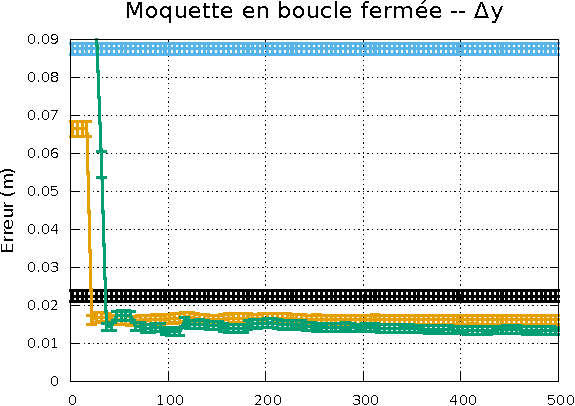
\includegraphics[type=pdf,ext=.pdf,read=.pdf,width=1.0\linewidth]{../plot/OdometryLWPR/carpet_close_convergence_y}
    \end{subfigure}
    \begin{subfigure}{0.29\paperwidth}
        \centering
        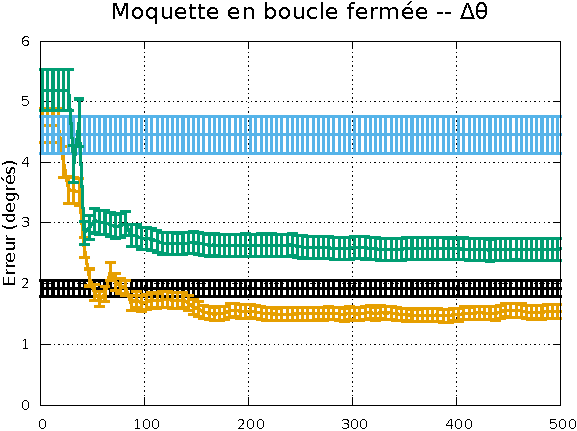
\includegraphics[type=pdf,ext=.pdf,read=.pdf,width=1.0\linewidth]{../plot/OdometryLWPR/carpet_close_convergence_yaw}
    \end{subfigure}
    %%%% Caption
    \caption{\label{fig:odometry_lwpr_convergence} 
        Comparaison des erreurs moyennes entre les déplacements proprioceptifs ou prédictifs et les déplacements mesurés par 
        la capture de mouvements en fonction de la taille de l'ensemble d'apprentissage (numéro $3$) des modèles LWPR.
        Les trois composantes $x,y,\theta$ ainsi que les différentes conditions sont comparées.
        Les intervalles de confiance à $95$\% sont également représentés.
    }
\end{figure}

Pour chaque contexte et après une phase d'optimisation des méta paramètres de LWPR 
(enregistrements numéros $1$ et $2$), les six
modèles de corrections des déplacements sont entrainés sur l'enregistrement numéro $3$.
Afin d'évaluer la vitesse et le nombre de points nécessaires à cet apprentissage, 
la figure \ref{fig:odometry_lwpr_convergence} représente la qualité de prédiction des modèles
en faisant varier le nombre de point d'apprentissage effectivement utilisé 
au sein des enregistrements numéros $3$.
La qualité de prédiction est évaluée sur la totalité des enregistrements de validations en calculant
l'erreur moyenne (et sa variance) entre la prédiction de déplacement et le déplacement mesuré 
par capture de mouvement.
Les différents graphiques comparent pour chacun des contextes et chacune des trois composantes
l'erreur de prédiction des déplacements avant et après correction.
Les déplacements avant correction ne dépendent pas de la taille de l'ensemble d'apprentissage.

Ces graphiques inspirent plusieurs commentaires :
\begin{itemize}
    \item Tous les apprentissages sont globalement terminés après avoir 
        présenté de l'ordre de $300$ points à LWPR (déplacements entre 
        deux changements de pied de support). 
        Pour un modèle linéaire, cela semble un nombre important 
        mais représente peu de données pour une méthode non paramétrique telle que LWPR.
    \item L'inspection des modèles LWPR après apprentissage révèle que le nombre
        de champs récepteurs (\textit{receptive field}) internes varie 
        selon les modèles entre $1$ et $5$ (voir section \ref{sec:odometry_non_parametric}).
        Ceci confirme que les fonctions effectivement construites sont toutes quasiment linéaires.
    \item Au cours de l'apprentissage, les données sont fournies à LWPR de manière séquentielle
        qui continuellement met à jour ses champs récepteurs en oubliant les données passées.
        C'est pourquoi l'erreur moyenne des déplacements corrigés continue de varier après
        un grand nombre de points appris.
    \item Il s'avère en pratique que la valeur absolue des erreurs moyennes varie selon
        l'enregistrement utilisé pour l'apprentissage. Une bonne couverture de l'espace
        des ordres de la marche est nécessaire pour que l'apprentissage soit satisfaisant.
    \item L'étape de correction ne permet pas de beaucoup améliorer la qualité de prédiction
        des rotations proprioceptives du robot. 
        En effet, sur toute la colonne de droite, les courbes noires (proprioception de base) 
        et oranges (proprioception corrigée) sont très proches.
        Les rotations avant et après corrections ont déjà toutes deux une faible erreur.
        Ceci vient du fait que l'orientation du robot pendant son fonctionnement est estimée 
        non pas au travers du modèle géométrique direct mais directement par intégration 
        des gyromètres de la centrale inertielle.
    \item A contrario, les rotations prédictives sans correction (courbes bleus) 
        ne sont pas précises et l'apport de la correction (courbes vertes) est importante.
    \item La phase de correction basée sur LWPR permet bien
        une amélioration de la qualité de prédiction des déplacements prédictifs
        et des déplacements proprioceptifs.
        Sur toutes les figures \ref{fig:odometry_lwpr_convergence}, 
        les courbes oranges sont en dessous (ou au même niveau
        pour la rotation) des courbes noires et les courbes vertes 
        en dessous des courbes bleus.
    \item On observe dans la plupart des cas que la correction permet 
        une réduction de la variance de l'erreur par rapport aux déplacements de base.
    \item On remarque que l'erreur des déplacements latéraux (colonne centrale) 
        prédictifs sans correction (bleu) est en valeur absolue plus élevée 
        en boucle fermée qu'en boucle ouverte.
        Ceci est directement un effet du processus de stabilisation principalement à l'oeuvre
        lors des pas chassés. Lorsqu'il se déclenche, le comportement prédit diffère grandement
        du comportement réel.
        Il semble que la correction parvienne à compenser ce phénomène\footnote{La déstabilisation
        et donc le déclenchement de la boucle fermée intervient le plus souvent sur 
        des grandes amplitudes de pas chassés. Il est possible que LWPR ait localement 
        appris ce phénomène. Il serait peut être intéressant d'étudier plus en détail cette région
        de l'espace d'état et sa non linéarité.}.
    \item Dans l'axe avant arrière (colonne de gauche) et en boucle ouverte
        (première et troisième ligne), les déplacements proprioceptifs possèdent une
        erreur plus grande que les déplacements prédictifs.
        Par exemple sur herbe artificielle, l'erreur moyenne des déplacements proprioceptifs
        monte à $0.032$~m alors que les déplacements prédictifs sont plus précis avec $0.022$~m.
        Ce résultat contre intuitif n'est pas simplement explicable.
        Ceci aurait pu être un effet du glissement affectant les pieds du robot mais
        les marches en boucle ouverte et fermée auraient été toutes deux affectées.\\
\end{itemize}

\begin{figure}[htbp]
    \centerfloat
    \begin{subfigure}{0.29\paperwidth}
        \centering
        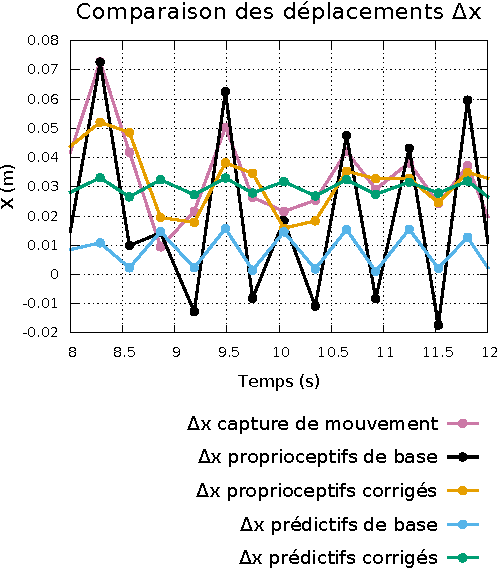
\includegraphics[type=pdf,ext=.pdf,read=.pdf,width=1.0\linewidth]{../plot/OdometryLWPR/grass_open_traj1_diff_x}
    \end{subfigure}
    \begin{subfigure}{0.29\paperwidth}
        \centering
        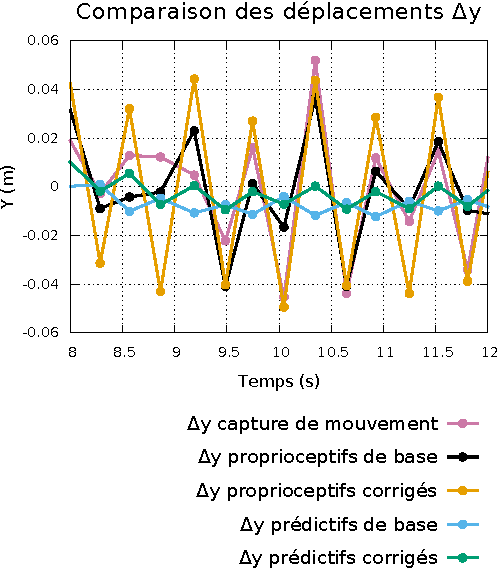
\includegraphics[type=pdf,ext=.pdf,read=.pdf,width=1.0\linewidth]{../plot/OdometryLWPR/grass_open_traj1_diff_y}
    \end{subfigure}
    \begin{subfigure}{0.29\paperwidth}
        \centering
        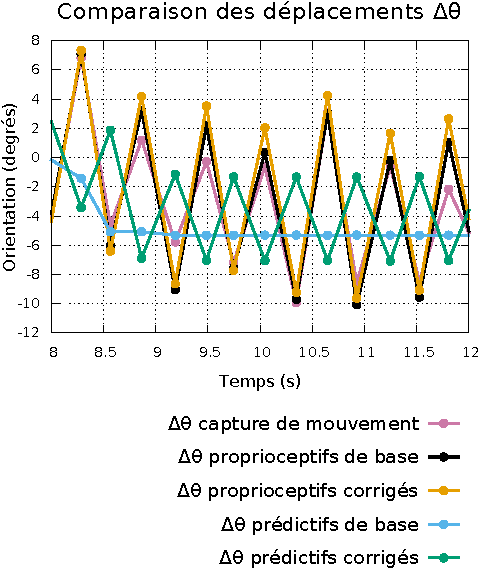
\includegraphics[type=pdf,ext=.pdf,read=.pdf,width=1.0\linewidth]{../plot/OdometryLWPR/grass_open_traj1_diff_yaw}
    \end{subfigure}
    \caption{\label{fig:odometry_lwpr_diff} 
        Illustration des trois composantes des déplacements du robot 
        entre deux changements de pied de support au cours du temps.
        Le déplacement mesuré par capture de mouvement, les déplacements 
        proprioceptifs et prédictifs sont montrés avant et après correction.
        Il s'agit d'un extrait de l'enregistrement numéro 4 
        sur herbe artificielle et en boucle ouverte.
    }
\end{figure}

\begin{figure}[htbp]
    \centerfloat
    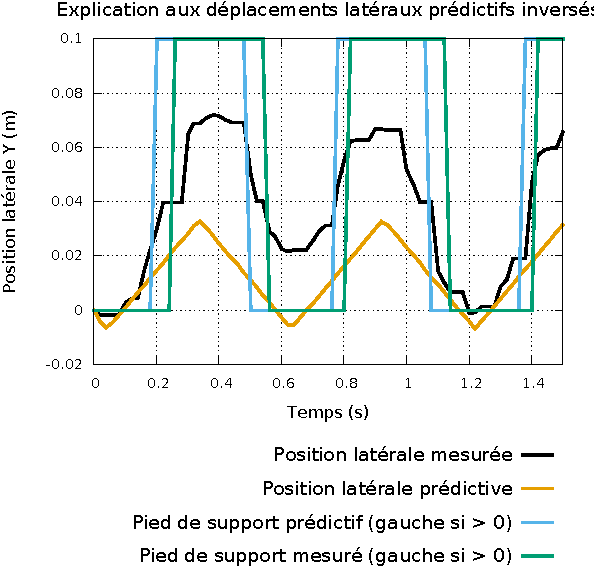
\includegraphics[type=pdf,ext=.pdf,read=.pdf,width=0.6\linewidth]{../plot/OdometryLWPR/grass_open_why_goal_lateral_diff}
    \caption{\label{fig:odometry_lwpr_why_goal_lateral_diff} 
        Représentation au cours du temps des pieds de support mesurés et prédits 
        et des position latérales du robot prédictives et mesurés par le système de capture de mouvement.
        Le différence entre les deux méthodes d'estimation du pied de support
        explique pourquoi les déplacements latéraux prédictifs semblent en opposition de phase.
    }
\end{figure}

Afin d'illustrer le résultat de l'apprentissage, la figure \ref{fig:odometry_lwpr_diff}
représente les trois composantes des différents types de déplacements du robots au cours du temps.
Pour chaque composante $\Delta x, \Delta y, \Delta \theta$, les déplacements mesurés par 
capture de mouvements et les déplacements proprioceptifs et prédictifs sont dessinés
avant et après correction.
Chaque point correspond à un déplacement à un moment du temps entre deux changements de pied de support.

Dans un premier temps, on vérifie bien que les déplacements proprioceptifs sont 
soumis à des oscillations d'une amplitude plus grande que les déplacements prédictifs.
On peut également remarquer que les oscillations des déplacements latéraux ($\Delta y$) 
prédictifs sans correction ainsi que les rotations ($\Delta \theta$) prédictives 
avant et après correction
semblent être en opposition de phase avec les autres déplacements.
Cela vient du fait que l'estimation du pied de support courant diffère entre 
l'odométrie proprioceptive et l'odométrie prédictive. 
De plus, les déplacements mesurés par capture de mouvement représentés sur 
la figure \ref{fig:odometry_lwpr_diff} sont ceux calculés en utilisant le pied de support
proprioceptif.
Ce comportement peut être compris plus en détail en observant 
la figure \ref{fig:odometry_lwpr_why_goal_lateral_diff}.

\subsubsection{Temps de calcul}

\includegraphics[type=pdf,ext=.pdf,read=.pdf,width=0.6\linewidth]{../schema/odometry_lwpr_perfs}

Les temps de calcul moyens de l'estimation en temps réel de l'odométrie observés 
à bord du robot (Intel Atom Z530) sont détaillés ci dessus.
Le temps de prédiction des trois modèles LWPR est ainsi inférieur à $3$~ms.
Comme mentionné plus haut, le nombre effectif de champs récepteurs dans les modèles
LWPR est en réalité très faible. 
Or, les temps de prédiction de LWPR sont linéaires en le nombre de ces
champs récepteurs.

Quant à la phase d'apprentissage, elle est ici réalisée hors-ligne 
sur un ordinateur bien plus puissant.
Avec un ensemble en entrée de l'ordre de $1000$ points, il ne faut que environ 
une seconde pour réaliser l'entrainement de chaque modèle LWPR.

\subsubsection{Réintégration des odométries et résultats\label{sec:odometry_lwpr_results}}

\begin{figure}[htbp]
    \centerfloat
    \vspace{-0.5cm}
    \begin{subfigure}{0.29\paperwidth}
        \centering
        \includegraphics[type=pdf,ext=.pdf,read=.pdf,width=1.0\linewidth]{../plot/OdometryLWPR/grass_open_traj1_pose}
    \end{subfigure}
    \begin{subfigure}{0.29\paperwidth}
        \centering
        \includegraphics[type=pdf,ext=.pdf,read=.pdf,width=1.0\linewidth]{../plot/OdometryLWPR/grass_open_traj2_pose}
    \end{subfigure}
    \newline
    \begin{subfigure}{0.29\paperwidth}
        \centering
        \includegraphics[type=pdf,ext=.pdf,read=.pdf,width=1.0\linewidth]{../plot/OdometryLWPR/grass_open_traj3_pose}
    \end{subfigure}
    \begin{subfigure}{0.29\paperwidth}
        \centering
        \includegraphics[type=pdf,ext=.pdf,read=.pdf,width=1.0\linewidth]{../plot/OdometryLWPR/grass_open_traj4_pose}
    \end{subfigure}
    \newline
    \begin{subfigure}{0.29\paperwidth}
        \centering
        \includegraphics[type=pdf,ext=.pdf,read=.pdf,width=1.0\linewidth]{../plot/OdometryLWPR/grass_open_traj5_pose}
    \end{subfigure}
    \begin{subfigure}{0.29\paperwidth}
        \centering
        \includegraphics[type=pdf,ext=.pdf,read=.pdf,width=1.0\linewidth]{../plot/OdometryLWPR/grass_open_traj6_pose}
    \end{subfigure}
    \caption{\label{fig:odometry_lwpr_trajs} 
        Comparaison sur six séquences de $50$ pas ($25$ cycles de marche) des différentes intégrations
        de l'odométrie avec la mesure externe de la trajectoire du robot.
        Ces séquences sont extraites de l'enregistrement numéro $4$ sur herbe artificielle et 
        avec un mouvement de marche en boucle ouverte. 
        Chaque point correspond à la pose du robot au changement de pied de support.
    }
\end{figure}

Après l'étape d'apprentissage et la correction des déplacements entre chaque pas, les différentes 
versions de l'odométrie du robot sont réintégrées à partir des déplacements et comparées.
Les enregistrements de validation sont découpés en séquences disjointes de $5$ à $60$ pas afin
d'y comparer la dérive de la pose du robot sur des mouvements relativement courts.
La figure \ref{fig:odometry_lwpr_trajs} donne l'exemple de six trajectoires typiques de $50$ pas
extraites de l'enregistrement numéro $4$ sur herbe artificielle et en boucle ouverte.
La trajectoire la moins précise est comme attendu l'odométrie prédictive non corrigée
étant donné que comme mentionné précédemment, elle tend à grandement sous estimer 
les distances et son estimation de l'orientation est également très imprécise.\\

\begin{figure}[htbp]
    \centerfloat
    \vspace{-0.5cm}
    \begin{subfigure}{0.37\paperwidth}
        \centering
        \includegraphics[type=pdf,ext=.pdf,read=.pdf,width=1.0\linewidth]{../plot/OdometryLWPR/grass_open_compare_cart}
    \end{subfigure}
    \begin{subfigure}{0.37\paperwidth}
        \centering
        \includegraphics[type=pdf,ext=.pdf,read=.pdf,width=1.0\linewidth]{../plot/OdometryLWPR/grass_open_compare_angle}
    \end{subfigure}
    \newline
    \begin{subfigure}{0.37\paperwidth}
        \centering
        \includegraphics[type=pdf,ext=.pdf,read=.pdf,width=1.0\linewidth]{../plot/OdometryLWPR/grass_close_compare_cart}
    \end{subfigure}
    \begin{subfigure}{0.37\paperwidth}
        \centering
        \includegraphics[type=pdf,ext=.pdf,read=.pdf,width=1.0\linewidth]{../plot/OdometryLWPR/grass_close_compare_angle}
    \end{subfigure}
    \newline
    \begin{subfigure}{0.37\paperwidth}
        \centering
        \includegraphics[type=pdf,ext=.pdf,read=.pdf,width=1.0\linewidth]{../plot/OdometryLWPR/carpet_open_compare_cart}
    \end{subfigure}
    \begin{subfigure}{0.37\paperwidth}
        \centering
        \includegraphics[type=pdf,ext=.pdf,read=.pdf,width=1.0\linewidth]{../plot/OdometryLWPR/carpet_open_compare_angle}
    \end{subfigure}
    \newline
    \begin{subfigure}{0.37\paperwidth}
        \centering
        \includegraphics[type=pdf,ext=.pdf,read=.pdf,width=1.0\linewidth]{../plot/OdometryLWPR/carpet_close_compare_cart}
    \end{subfigure}
    \begin{subfigure}{0.37\paperwidth}
        \centering
        \includegraphics[type=pdf,ext=.pdf,read=.pdf,width=1.0\linewidth]{../plot/OdometryLWPR/carpet_close_compare_angle}
    \end{subfigure}
    \caption{\label{fig:odometry_lwpr_compare} 
        Dérive moyenne de la position cartésienne et de l'orientation des différentes intégrations 
        de l'odométrie en fonction du nombre de pas effectués par le robot.
        Les intervalles de confiance à $95$\% sont donnés.
    }
\end{figure}

Enfin, les résultats principaux de cette étude sont résumés par l'analyse statistique de 
la précision des différentes méthodes sur les quatre contextes et sont présentés par 
la figure \ref{fig:odometry_lwpr_compare}.
Pour chaque contexte et chaque méthode, l'erreur moyenne et la variance entre la position 
cartésienne et angulaire finale estimées du robot et celles fournies par la capture de 
mouvement sont comparées en fonction du nombre de pas afin d'exposer l'évolution de la dérive.
Les valeurs numériques des dérives cartésiennes après $40$ pas sont extraites et regroupées dans 
le tableau \ref{tab:odometry_lwpr_values}.
Cet valeurs sont également représentées graphiquement sur la figure \ref{fig:odometry_lwpr_values_bar}.

Les quelques commentaires généraux suivant peuvent être fait :
\begin{itemize}
    \item Comme remarqué précédemment, l'apprentissage n'apporte 
        que très peu d'amélioration pour l'orientation proprioceptive.
        Sur la colonne de droite du graphique \ref{fig:odometry_lwpr_compare},
        les courbes noires et oranges sont quasiment confondues.
    \item Dans les deux cas de l'odométrie proprioceptive et prédictive, la correction
        améliore significativement la précision de l'intégration de la position du robot.
        Sur le tableau \ref{tab:odometry_lwpr_values}, on observe que pour 
        l'odométrie proprioceptive, l'erreur est divisée par $2.9$, $1.8$, $2.0$ ou $1.49$
        alors que l'erreur de l'odométrie prédictive est divisée par $4.4$, $2.32$, $2.6$ ou $1.6$
        selon les différents contextes.
    \item Dans tous les cas après correction, l'odométrie proprioceptive est en valeur
        absolue la plus précise.
    \item La correction tend à réduire la variance par rapport à l'estimation de base.
        Par exemple sur herbe artificielle et en boucle ouverte, la taille des intervalles
        de confiance à $95$\% passe de $\pm0.050$~m à $\pm0.037$~m pour la prédiction
        et de $\pm0.037$~m à $\pm0.030$~m pour la proprioception.
    \item On observe après $40$ ou $50$ pas une modification de la tendance des courbes.
        L'erreur ne semble plus augmenter à la même vitesse.
        Il s'agit en réalité d'un biais statistique induit par la petite taille de notre
        zone de capture. Le robot piloté manuellement parcours malheureusement de nombreuses boucles.
        Or, le temps de parcours du diamètre de la zone en ligne droite est justement de l'ordre de 
        $15$ secondes (soit $25$ cycles de marche et $50$ pas).
        Par exemple dans le cas d'une trajectoire fermée, une odométrie 
        qui sous-estimerait les distances mais pas les rotations reviendrait 
        bien au point de départ et obtiendrait alors un bon score.
        Il n'est ainsi pas fiable de considérer les résultats sur 
        des trajectoires trop longues.
        Ce phénomène de biais possible avait déjà évoqué par \cite{antonelli_calibration_2005}.\\
\end{itemize}

Pour terminer, une comparaison plus fine des différents contextes nous apprend 
les quatre faits intéressants suivants :
\begin{enumerate}
    \item Si l'on considère les estimations de l'odométrie sans correction, 
        l'activation du processus de stabilisation en boucle fermée de la marche à pour effet 
        de réduire l'erreur en cartésienne à la fois prédictive et proprioceptive.
        Par exemple sur moquette, l'erreur passe de $0.504$~m à $0.435$~m pour la prédiction
        et de $0.341$~m à $0.228$~m pour la proprioception.
        Le processus de stabilisation améliore la robustesse de la marche en évitant 
        au robot d'entrer dans des oscillations latérales parasites.
        Une interprétation possible est que le comportement réel du système est alors plus proche 
        de sa dynamique de référence et les deux méthodes d'estimation 
        de base sont ainsi plus efficaces.
    \item Toujours sans correction, marcher sur de l'herbe artificielle 
        entraine une augmentation de la dérive de l'odométrie prédictive par rapport au fait de
        marcher sur de la simple moquette.
        En boucle ouverte, $0.701$~m sur herbe contre $0.504$~m sur moquette et 
        $0.566$~m contre $0.435$~m en boucle fermée.
        Par contre, l'odométrie proprioceptive (non corrigée) n'est pas 
        significativement affectée.
        En boucle ouverte, $0.342$~m sur herbe et $0.341$~m sur moquette.
        En boucle fermée, $0.222$~m sur herbe et $0.228$~m sur moquette.
        Ceci peut s'expliquer par le fait que les brins épais de l'herbe artificielle
        induisent un fort frottement contre les pieds du robot pendant leur déplacement.
        Ce frottement pourrait alors affecter la position réelle à laquelle se repose le pied.
        Les déplacements prédictifs en serait donc influencés.
        À l'inverse, l'odométrie se basant sur les encodeurs des moteurs et estimant géométriquement
        le déplacement réel des jambes prendrait en compte ce phénomène.
    \item On constate également qu'après correction, l'odométrie prédictive
        est plus précise avec un mouvement de marche en boucle ouverte qu'avec un mouvement
        de stabilisation en boucle fermée.
        Sur herbe artificielle, l'erreur moyenne passe de $0.165$~m en boucle ouverte 
        à $0.243$~m en boucle fermée.
        Le processus de stabilisation déclenche un comportement qui ne peut pas être 
        correctement prédit uniquement à partir des ordres de la marche. 
        Comme le déplacement du robot s'en trouve plus stable mais affecté, 
        l'odométrie prédictive en pâtit.
        À noter qu'en boucle ouverte, l'odométrie prédictive après correction
        parvient même à être plus précise que l'odométrie de base proprioceptive.
    \item Pour finir, on remarque que les deux odométries corrigées 
        sont un petit peu plus précises sur herbe artificielle que sur moquette.
        Par exemple en boucle ouverte et pour la proprioception, l'erreur de
        l'odométrie corrigée passe de $0.170$~m sur moquette à $0.118$~m sur herbe artificielle.
        Il s'avère qu'en pratique, les crampons des pieds du robot s'enfoncent dans 
        l'épaisseur de l'herbe et s'y maintiennent relativement bien.
        Il est fort possible que les glissements des pieds par rapport au sol soit ainsi
        plus présents sur la moquette que sur l'herbe pendant la marche.
        Or, les glissements non déterministes sont l'une des causes principales de la dérive 
        de l'odométrie car ils ne sont mesurés par aucun capteur proprioceptif.
\end{enumerate}

\begin{table}[htb!]
    \centerfloat
    \small
    \begin{tabular}{|l|l|l|p{2.5cm}|p{2.5cm}|}
        \hline
        Surface & Marche & Type & Distance cartésienne moyenne (m) & Intervalle de confiance à 95\% (m)\\
        \hline
        Herbe & Ouverte & Prédiction base & $0.701$ & $\pm0.050$\\
        Herbe & Ouverte & Prédiction corrigée & $0.165$ & $\pm0.037$\\
        Herbe & Ouverte & Proprioception base & $0.342$ & $\pm0.037$\\
        Herbe & Ouverte & Proprioception corrigée & $0.118$ & $\pm0.030$\\
        \hline
        Herbe & Fermée & Prédiction base & $0.566$ & $\pm0.042$\\
        Herbe & Fermée & Prédiction corrigée & $0.243$ & $\pm0.039$\\
        Herbe & Fermée & Proprioception base & $0.222$ & $\pm0.029$\\
        Herbe & Fermée & Proprioception corrigée & $0.125$ & $\pm0.018$\\
        \hline
        Moquette & Ouverte & Prédiction base & $0.504$ & $\pm0.043$\\
        Moquette & Ouverte & Prédiction corrigée & $0.192$ & $\pm0.034$\\
        Moquette & Ouverte & Proprioception base & $0.341$ & $\pm0.028$\\
        Moquette & Ouverte & Proprioception corrigée & $0.170$ & $\pm0.021$\\
        \hline
        Moquette & Fermée & Prédiction base & $0.435$ & $\pm0.090$\\
        Moquette & Fermée & Prédiction corrigée & $0.270$ & $\pm0.071$\\
        Moquette & Fermée & Proprioception base & $0.228$ & $\pm0.044$\\
        Moquette & Fermée & Proprioception corrigée & $0.149$ & $\pm0.025$\\
        \hline
    \end{tabular}
    \caption{\label{tab:odometry_lwpr_values}
        Dérive moyenne et intervalle de confiance des différentes odométries sur 
        les quatre contextes après $40$ pas ($20$ cycles de marche)
        soit environ $12$~s de marche.
        Ces valeurs sont représentées graphiquement sur 
        la figure \ref{fig:odometry_lwpr_values_bar}.
    }
\end{table}

\begin{figure}[htb!]
    \centerfloat
    \includegraphics[type=pdf,ext=.pdf,read=.pdf,width=0.7\linewidth]{../plot/OdometryLWPR/comparison_values}
    \caption{\label{fig:odometry_lwpr_values_bar} 
        Rerpésentation graphique des valeurs données dans le tableau \ref{tab:odometry_lwpr_values}.
        Dérive moyenne et intervalle de confiance des différentes odométries sur 
        les quatre contextes après $40$ pas ($20$ cycles de marche)
        soit environ $12$~s de marche.
    }
\end{figure}

\subsection{Discussion et conclusion\label{sec:odometry_lwpr_limits_and_conclusions}}

Comme le détaillent les différents graphiques de corrélations, le mouvement 
des petits robots humanoïdes est soumis à de nombreuses perturbations.
Le système mécanique complexe subit d'importants jeux des engrenages, 
chocs et souffre de problèmes d'asservissement.
De plus, la déformation des pièces mécaniques au cours du temps fait qu'il
est difficile d'avoir un modèle géométrique précis de ce système.
Outre le glissement, principale source de dérive chez les robots à roues 
car non mesuré, l'estimation de la pose réelle des pieds par rapport au sol
est également délicate.
Les déséquilibres de la marche entrainent souvent le ou les pieds de support
à ne pas être à plat sur le sol mais plutôt à reposer temporairement 
sur uniquement un ou deux crampons.
Ces phases de doubles supports ne sont pas ici modélisées bien qu'elles
soient la cause de glissement lorsque les deux pieds forcent 
l'un contre l'autre sur le sol.

En plus de tous ces phénomènes, il faut y ajouter le bruit et les 
limitations inhérent à nos capteurs.
Les capteurs de pression ne sont que modérément résilients, 
la résolution des encodeurs des moteurs est limitée et le filtrage
de la centrale inertielle impose elle même un compromis entre bruit et réactivité.
À noter de plus qu'une analyse quantitative de la précision et du bruit du système de
capture de mouvement pendant le suivi d'un objet \textit{en mouvement} 
n'a pas été conduit.

La somme de tous ceci explique pourquoi le lien entre les ordres donnés au générateur de marche
et le déplacement effectif du robot est empreint d'un bruit conséquent et renseigne sur
la difficulté du problème.\\

Dans sa forme actuelle, la méthode d'apprentissage proposée reste a priori dépendante des paramètres
du mouvement de marche (listés à la section \ref{sec:walk}).
Malheureusement, il est souvent nécessaire pour conserver une bonne stabilité d'adapter ses
paramètres à la surface de marche, ou simplement pour compenser les petites déformations
mécaniques du robot.
Dans cette étude, les mêmes paramètres de marche ont été utilisés à la fois pour
les expérimentations sur herbe artificielle et sur moquette. Leur influence n'a pas été analysée.
Les paramètres utilisés ont initialement été ajustés spécifiquement pour l'herbe artificielle.
Il est ainsi possible que le mouvement de marche aurait pu être plus stable sur moquette si 
les paramètres du générateur avaient été réajustés sur cette surface.
Les comparaisons de surfaces présentées ci-dessus ne sont donc valides qu'à 
paramètres de la marche fixés. 
Les résultats sont potentiellement différents lorsque la marche est \og optimisée \fg comme
elle le devrait pour chaque surface.

Il est également manifeste que le pilotage du robot à la manette bien que pratique 
n'est pas idéal pour explorer correctement l'espace d'actions.
Il s'avère sans surprise que la qualité de couverture de l'enregistrement utilisé 
pour l'apprentissage est essentiel. 
L'apprentissage sur un enregistrement où les ordres envoyés à la marche 
ne sont pas assez diversifiés converge vers une mauvaise correction et l'odométrie 
résultante peut alors être moins bonne que l'odométrie de base.

Grâce au système de capture de mouvement, la mesure précise de la pose du robot
dans le monde est possible. Cette mesure permettant d'en déduire les déplacements 
à chaque pas est indispensable à la méthode proposée.
Ainsi, une fois le système mis en place, un enregistrement de moins 
de cinq minutes est suffisant pour réaliser l'apprentissage.
Cependant, ce système de six caméras est relativement lourd à déployer, 
à calibrer et impose de nombreuses contraintes de par la taille réduire de sa zone de capture.
Bien que ce système soit au cœur de la méthode proposée, c'est également son principal défaut.
Il est malheureusement inenvisageable en pratique de transporter puis de mettre 
en place ce système dans les conditions logistiques imposées par la compétition RoboCup.
Or il est également essentiel de pouvoir sur place réajuster les différents paramètres
du mouvement de marche des robots.
Sans une étude plus approfondie sur l'influence des paramètres de la marche sur l'odométrie,
et en l'espérant négligeable, cette méthode ne peut être employée à la calibration 
de l'odométrie dans un contexte RoboCup.

Néanmoins, les informations récoltées grâce à ce système de capture de mouvement sont riches 
et cette étude apporte des éléments importants sur la compréhension du problème.
Étant donné l'importance du bruit observé dans les corrélations, il semble difficile 
d'envisager un modèle de correction beaucoup plus complexe que linéaire ou quadratique.
Le choix d'utilisation de la régression non paramétrique LWPR est à postériori non justifié.
Il serait d'ailleurs intéressant de comparer sur ces mêmes données les performances 
obtenues par un simple modèle linéaire.

Même avec l'utilisation de régressions non paramétriques, les atouts de l'algorithme 
LWPR permettent d'atteindre de faibles temps de calculs.
Mesurés sur le petit processeur embarqué du robot, ces temps de calcul sont suffisant 
pour autoriser l'estimation et la correction de l'odométrie à $100$~Hz.
À noter tout de même qu'avec des modèles purement linéaires, vraisemblablement de qualités similaires,
les temps de calculs de prédiction et d'apprentissage deviendraient alors négligeables.\\

Il est intéressant de comparer les résultats de cette étude avec les techniques d'odométrie visuelles
qui se sont depuis une dizaine d'années particulièrement développées sur les robots humanoïdes 
(voir la littérature section \ref{sec:biblio_odometry}).
Un des exemples récents les plus approfondie d'odométrie visuelle est 
réalisé par \cite{oriolo_humanoid_2016} sur le robot NAO.
Les auteurs se basent sur d'une part, le modèle géométrique direct et les capteurs
de pression du NAO (capteurs FSR, \textit{Force Sensing Resistor}) et d'autre part 
sur la caméra et le suivi de points de repères extérieurs. 
Un filtrage de Kalman mélange les deux estimations et calcul les déplacements du robot.
Sans phase d'apprentissage des erreurs systématiques, 
ils annoncent qu'après une marche en ligne droite 
d'une quarantaine de pas (environs $25$~s), la dérive de la position n'est que de l'ordre de $0.03$~m.
Pour comparaison, la méthode présentée ici dans des conditions similaires 
dérive en moyenne de $0.12$~m.
À noter néanmoins que la caméra et le filtre de Kalman ont besoin d'être calibrés et que 
le traitement des images n'est pas réalisé à bord du robot mais est déporté sur une 
station de calcul plus puissante.

Contrairement aux approches visuelles, la méthode proposée ici n'a aucun moyen de capturer
les glissements des pieds sur le sol non systématiques.
L'analyse de la caméra en suivant des éléments externes s'affranchit également des problèmes
liés à la calibration et au filtrage de la centrale inertielle ainsi qu'à la détermination 
du pied de support.

Pour conclure en ce qui concerne l'odométrie proprioceptive, les approches visuelles 
sont au vu de leur précision et de leur versatilité à préférer 
s'il est possible de les mettre en oeuvre.
Il est toutefois possible de combiner la calibration proprioceptive 
et l'analyse visuelle pour encore améliorer la précision et la robustesse de l'estimation.
Cependant dans le contexte de la compétition RoboCup,
il n'est pas certain que le gain de précision apporté soit réellement utile ; 
surtout au regard de l'effort nécessaire à la maintenance simultanée des deux techniques.
Si par contre pour des raisons de limitations de la puissance de calcul disponible 
ou si l'environnement visuel ne fournit pas suffisamment de points de repères pour 
assurer une analyse robuste, la méthode proposée reste une bonne alternative.

Au final, le principal intérêt comparatif de cette technique est bien la construction d'un
modèle prédictif de déplacement dont la précision est grandement améliorée par rapport
à l'estimation prédictive de base ; et notamment avec une marche en boucle ouverte. 
Ce point n'est pas traité par les méthodes visuelles mais a déjà été abordé 
sur un robot humanoïde par \cite{schmitz_learning_2010} dans un contexte 
très proche (système de capture de mouvement, régressions linéaires). 
Seule la prédiction des déplacements à chaque pas est abordée mais la précision de 
l'intégration de l'odométrie résultante n'est pas étudiée.
Les auteurs annoncent une erreur moyenne de prédiction des déplacements $\Delta x$
de l'ordre de $0.13$~m puis analyse l'influence du transfert de l'apprentissage 
entre différents robots.
La suite naturelle à donner à cette étude est donc son application
à la planification de trajectoire.
L'objectif étant de réduire l'effort d'asservissement de la trajectoire
nécessaire pour atteindre une pose cible en prenant en compte a priori 
les perturbations affectant le déplacement réel du robot.

